\section{Introduzione}
Nella terza iterazione è stato approfondito e implementato l'algoritmo portante del sistema: l'algoritmo di Discover permette di ``Scoprire" nuova 
musica e nuovi utenti in base alle preferenze dell'utente.
In seguito si procede con la parte di Testing, quindi analisi statica (tramite Electron) e dinamica (sia di backend sia tramite Coverage.py).


\section{Implementazione del caso d'uso}
\subsection{UC19 -- ``Discover''}
\begin{itemize}
    \item \textbf{Actor:} Utente base.
    \item \textbf{Precondition:} L'utente deve aver effettuato il log in.
    \item \textbf{Postcondition:} L'utente può scoprire nuovi brani e aggiungere nuovi amici secondo i suggerimenti dell'algoritmo. 
    \item \textbf{Base Sequence:}
    \begin{itemize}
        \item \textbf{1.} L'utente, dopo aver effettuato il log in, clicca su Discover dal menu a sinistra.
        \item \textbf{2.} L'utente naviga nella pagina dei brani e amici suggeriti.
        \item \textbf{3.} L'utente ha correttamente eseguito l'operazione.
    \end{itemize}
    \item \textbf{Exception Sequence:} Connessione fallita.
    \begin{itemize}
        \item Nel caso di connessione fallita si ritorna al passo 1 della Base Sequence del caso d'uso \textbf{UC1}.
    \end{itemize}
\end{itemize}
\vspace{1cm}

\section{UML Component Diagram}
In figura sono presenti tutte le interfacce
relative alle componenti implementate in questa iterazione, 
ovvero Amici e Discover (parte relativa all'algoritmo).
\begin{figure}[H]
    \centering
    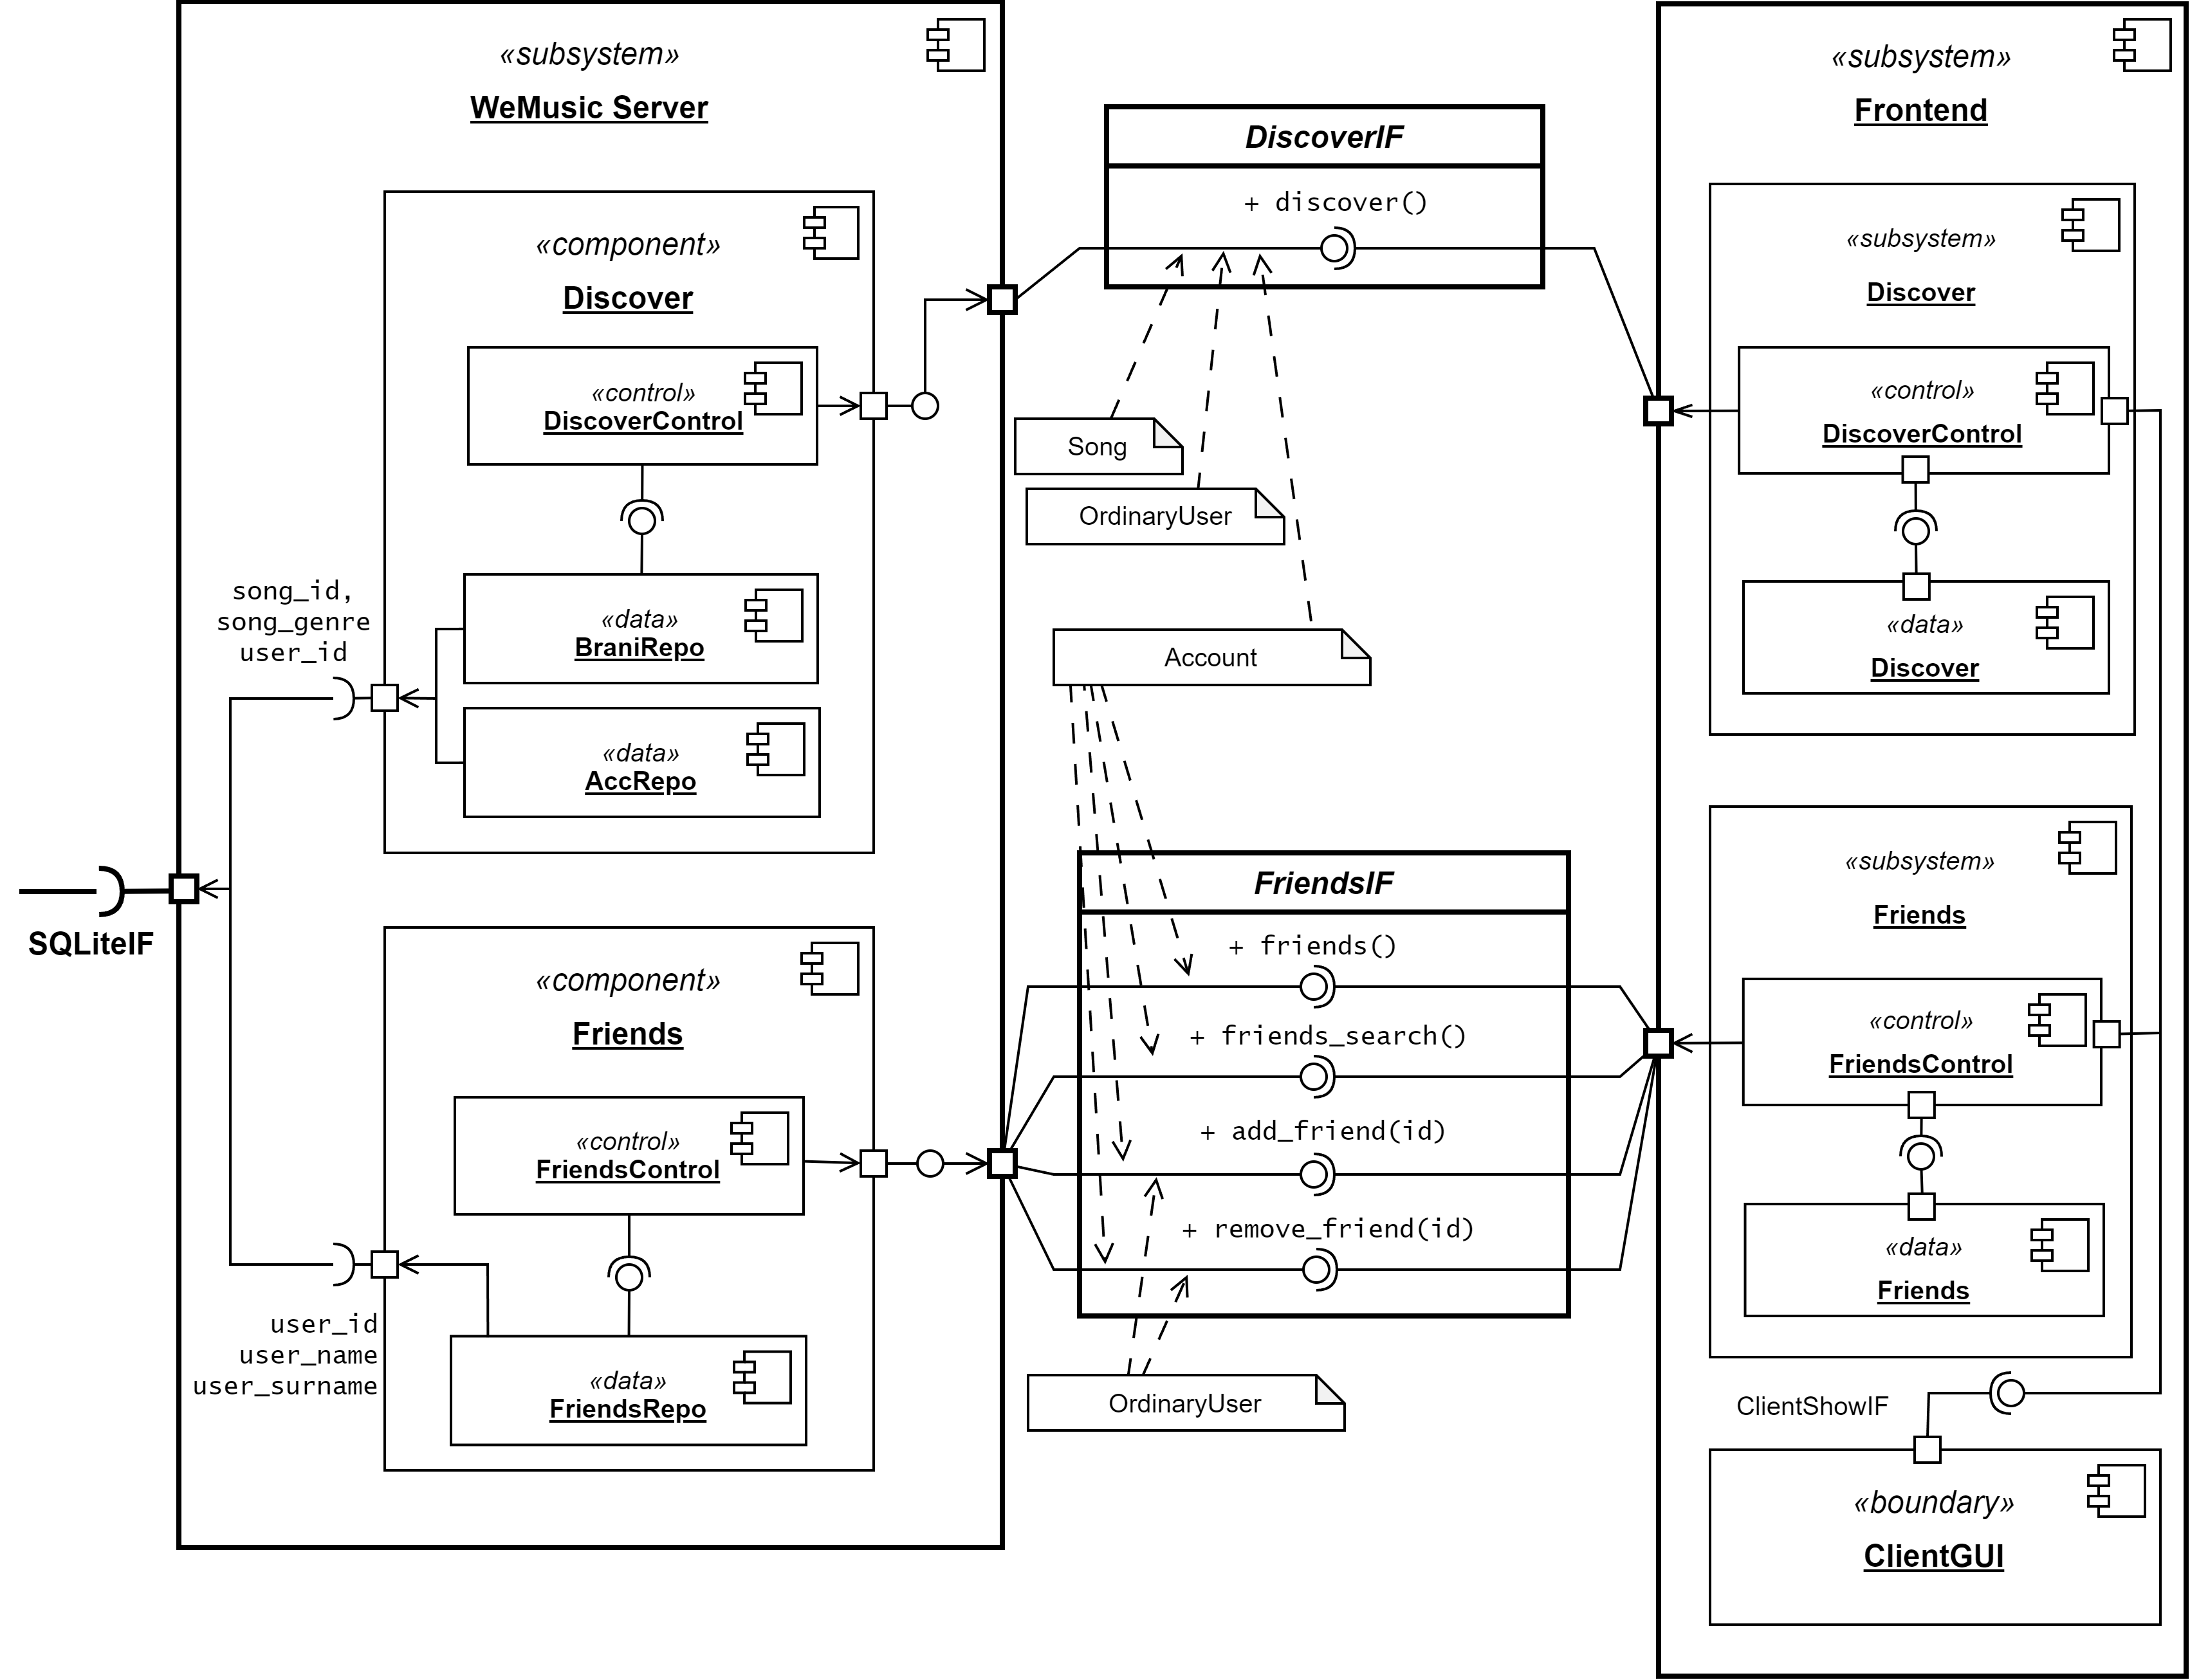
\includegraphics[scale=0.62]{component_diagram_ver5_5.png} 
    \caption{UML Component Diagram}
    \label{fig-uml-component-diag_5}
\end{figure}

\newpage
\section{Descrizione dell'algoritmo}
L'algoritmo di Discover è stato ideato per offrire all'utente un'esperienza completa di riproduzione e scoperta di nuova musica, unendo a ciò la 
componente social: in questo modo si permette all'utente di conoscere nuove persone che condividono con lui i propri gusti musicali. 

Questo tipo di algoritmo 
tiene traccia dei generi preferiti dell'utente e lo utilizza per suggerire musica simile, ma non solo: allo stesso modo riesce a suggerire 
una lista di utenti che hanno gusti simili all'utente loggato, in modo da poterli aggiungere alla propria lista di amici.  

Le variabili e i fattori tenuti in considerazione per lo sviluppo dell'algoritmo di Discover sono i seguenti: 
\begin{itemize}
    \item Il genere favorito dell'utente, ottenuto da un'analisi dei suoi brani preferiti;
    \item L'età dell'utente;
    \item Il sesso dell'utente.
\end{itemize}

\vspace{1cm}
\section{Funzionamento dell'algoritmo}
Il funzionamento dell'algoritmo si basa su una previsione Machine Learning, tramite la libreria \textbf{Pandas} di Python;
il nome fa riferimento sia a ``Panel Data" che ``Python Data Analysis", infatti è una libreria molto utilizzata per lavorare 
con dataset: tramite le sue molteplici funzioni consente di analizzare, pulire, esplorare e manipolare i dati, definendo 
conclusioni basate su teorie statistiche. 

Come anticipato, in base al genere preferito dell'utente, il suo sesso e la sua età, l'algoritmo suggerisce dei brani ricavandoli 
da un dataset, filtrandoli secondo le variabili sopracitate. Al termine dell'esecuzione l'algoritmo mostrerà un elenco di brani e amici suggeriti.

Gli step di funzionamento dell'algoritmo possono essere così riassunti: 
\begin{itemize}
    \item Inizialmente, viene creato un oggetto account contenente le informazioni relative all'account dell'utente loggato, che ci serviranno in seguito; 
    viene passato il parametro \textbf{request} che è quello che contiene le informazioni di interesse, ovvero l'età e il sesso (1=maschio, 0=femmina). 
    In seguito viene utilizzato un training set (\textbf{utenti.csv}) sul quale allenare la stima, contenente le informazioni degli utenti 
    necessarie per estrapolare le variabili: quelle di input includono il sesso e l'età dell'utente, quella di output contiene solo 
    il genere preferito (ciò che suggerirà l'algoritmo). 

    \item Dopo aver creato queste due tabelle viene istanziato il modello previsionale tramite il comando \textbf{DecisionTreeClassifier}, un comando 
    della libreria Pandas che permette, dandogli in input le variabili considerate, di fittare il modello che le lega. 
    
    \item Viene quindi fittato il modello tramite il comando \textbf{modello.fit(...)}, che si allenerà sulle variabili scelte (età e sesso), per restituire 
    il risultato (genere preferito). 

    \item In seguito verrà effettuata la predizione inserendo le informazioni relative all'utente loggato tramite la funzione \textbf{modello.predict}, ed 
    infine viene memorizzata la previsione relativa solo alla variabile di genere musicale. 
    
\end{itemize}

\vspace{1cm}
\subsection{Discover: Suggerimento brano}
Nella parte successiva dell'algoritmo Discover si effettua un semplice filtro su tutte le canzoni presenti nel database del sistema e vengono
 selezionate solo quelle che rispettano il genere target restituito dall'algoritmo Discover; vengono in seguito salvate in una 
 lista e proposte all'utente, che sarà in grado di navigare e selezionare quale scaricare o aggiungere ai preferiti o ad una playlist. 

 
\newpage
\subsection{Discover: Suggerimento amici}
Nell'ultima parte dell'algoritmo Discover viene seguito un processo più meccanico: facendo ancora riferimento al genere target 
individuato nella parte iniziale dell'algoritmo, viene estrapolata una lista di amici suggeriti per l'utente. 

Inizialmente viene creata una lista amici vuota, vengono salvate le informazioni relative dell'utente loggato, vengono quindi 
selezionati tutti gli utenti presenti nella lista amici (in modo da escluderli in seguito nell'algoritmo).
Dopo aver creato una lista degli identificativi, tramite un ciclo for each vengono selezionati gli utenti nel database 
sfogliando per ognuno le canzoni preferite, al fine di salvare il genere di ogni canzone in una variabile y.

Condizione per rientrare negli utenti suggeriti:
\begin{itemize}
    \item L'utente analizzato (nel database) non deve essere l'utente loggato, ovvero devono avere id diversi;
    \item L'utente analizzato (nel database) non deve essere amico dell'utente loggato, ovvero il suo id non deve essere presente 
    nella lista amici;
    \item All'utente analizzato (nel database) deve piacere almeno una canzone che abbia lo stesso genere target dell'algoritmo.

\end{itemize}

Nel context viene poi passata la lista creata con gli utenti selezionati dal database, in modo da permettere all'utente di poter
navigare fra gli utenti ed, eventualmente, aggiungerli fra gli amici. 




\newpage

\section{Studio della complessità}

\subsection{Algortimo Parte I}
\vspace{0.5cm}
\subparagraph{Pseudocodice}
Pseudocodice della prima parte dell'algoritmo, relativa all'inizializzazione 
e all'individuazione del genere target. 
% codice 1
%\begin{figure}[H]
%    \centering
%    \begin{center}
%    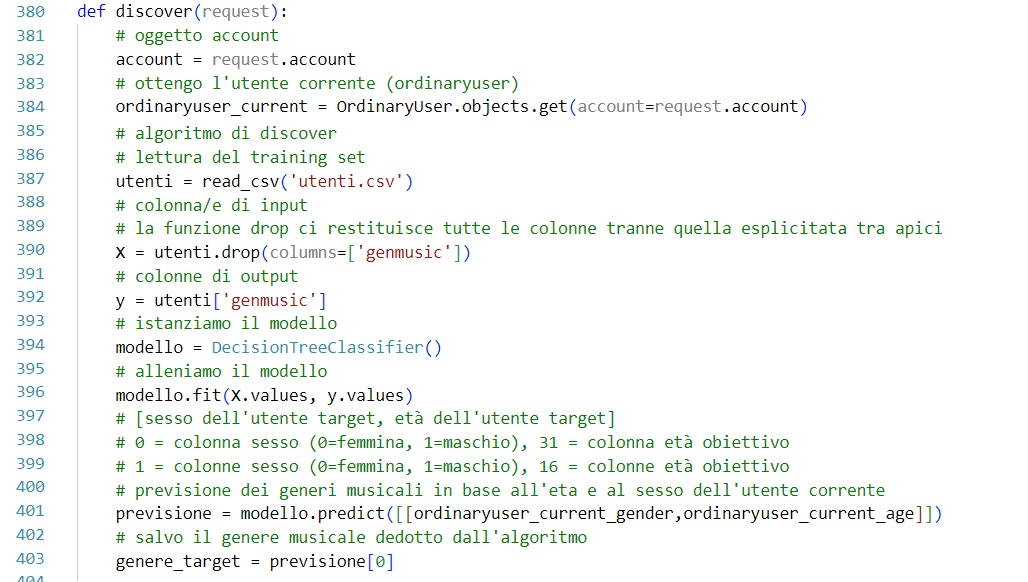
\includegraphics[scale=0.5]{images/alg1_v2.jpg}
%    \end{center}
%    \caption{Codice (parte I)}
%    \label{fig-codice1}
%\end{figure}

% pseudocodice 1
\begin{algorithm}
    \caption{Step 1 - Inizializzazione}
    \SetAlgoLined
    \LinesNumbered
    \SetKwProg{myalg}{algoritmo}{ begin}{end}
    \myalg{Discover($curr\_gender$, $curr\_age$)}{
        \BlankLine
        \BlankLine
        \textbf{/* Creazione oggetto account */}\

        \textbf{do}{
            $account \leftarrow request.account$
        }
        \BlankLine
        \BlankLine
        
        \textbf{/* Memorizzazione utente corrente */}\\
            \textbf{do}{
            $curr\_user \leftarrow curr\_user.\underline{get}()$
        }
        \BlankLine
        \BlankLine
        \textbf{/* Lettura training set degli utenti.csv */}\
            
        \textbf{do}{
           $utenti \leftarrow read\_csv('utenti.csv')$
        }
        \BlankLine
        \BlankLine
        \textbf{/* Creazione colonna di input della previsione */}\
            
        \textbf{do}{
            $X \leftarrow utenti.\underline{drop}(columns=['genmusic'])$
        }
        \BlankLine
        \BlankLine
        \textbf{/* Creazione colonna di output della previsione */}\
            
        \textbf{do}{
            $y \leftarrow utenti['genmusic'] $
        }
        \BlankLine
        \BlankLine
        \textbf{/* Creazione istanza del modello */}\
            
        \textbf{do}{
            $ modello \leftarrow \underline{DecisionTreeClassifier}()$
        }
        \BlankLine
        \BlankLine
        \textbf{/* Allenamento del modello sui dati */}\
            
        \textbf{do}{
            $ modello.\underline{fit}(X.values, y.values)$
        }
        \BlankLine
        \BlankLine
        \textbf{/* Previsione dei generi */}\
            
        \textbf{do}{
            $previsione \leftarrow modello.\underline{predict}(curr\_gender, curr\_age)$
        }
        \BlankLine
        \BlankLine
        \textbf{/* Memorizzazione del genere target */}\

        \textbf{do}{
            $genere\_target \leftarrow previsione[0]$
        } 

        \BlankLine
        \textbf{...}
        \BlankLine
        \KwResult{Genere target}
        \BlankLine
        
    }
\end{algorithm}

% flowchart 1
\newpage

%\subparagraph{Diagramma di flusso} 
%Diagramma di flusso della prima parte dell'algoritmo.
%\begin{figure} [H]
%    \centering
%    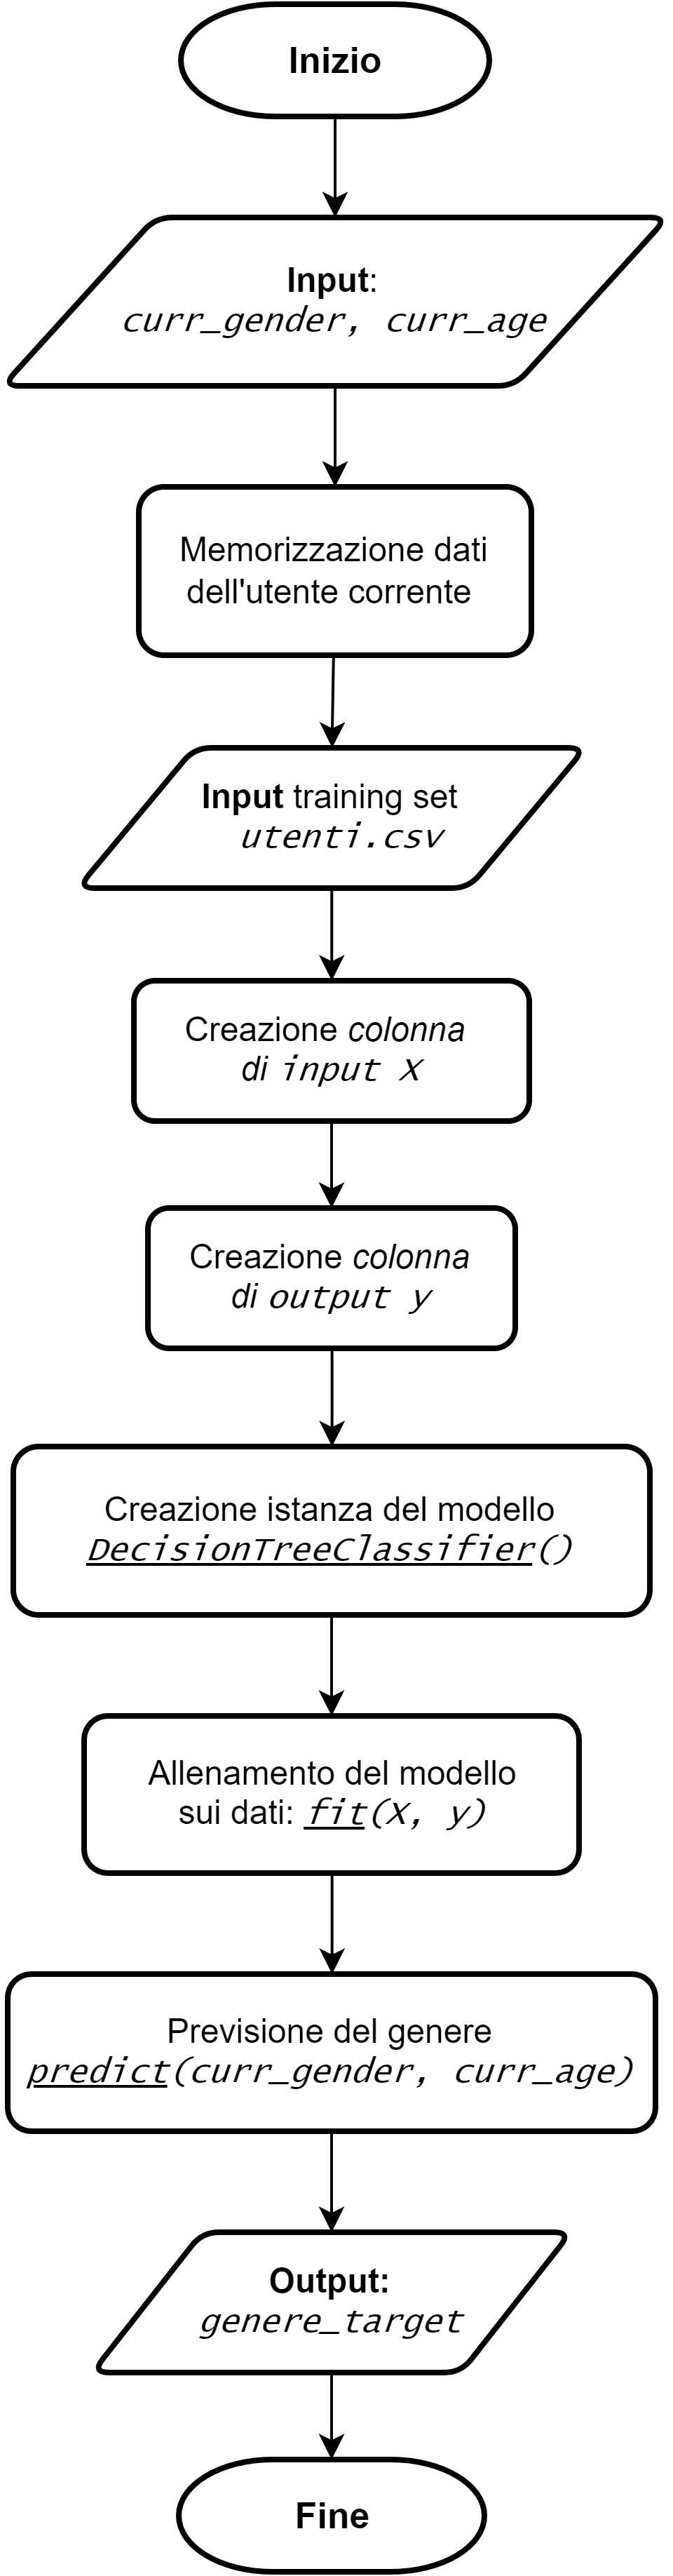
\includegraphics[scale=0.7]{images/flowchart-Parte I.png}
%    \caption{Flowchart (parte I)}
%    \label{fig-fc1}
%\end{figure}

\subparagraph{UML Activity Diagram}
Diagramma delle attività della prima parte dell'algoritmo.
\begin{figure} [H]
    \centering
    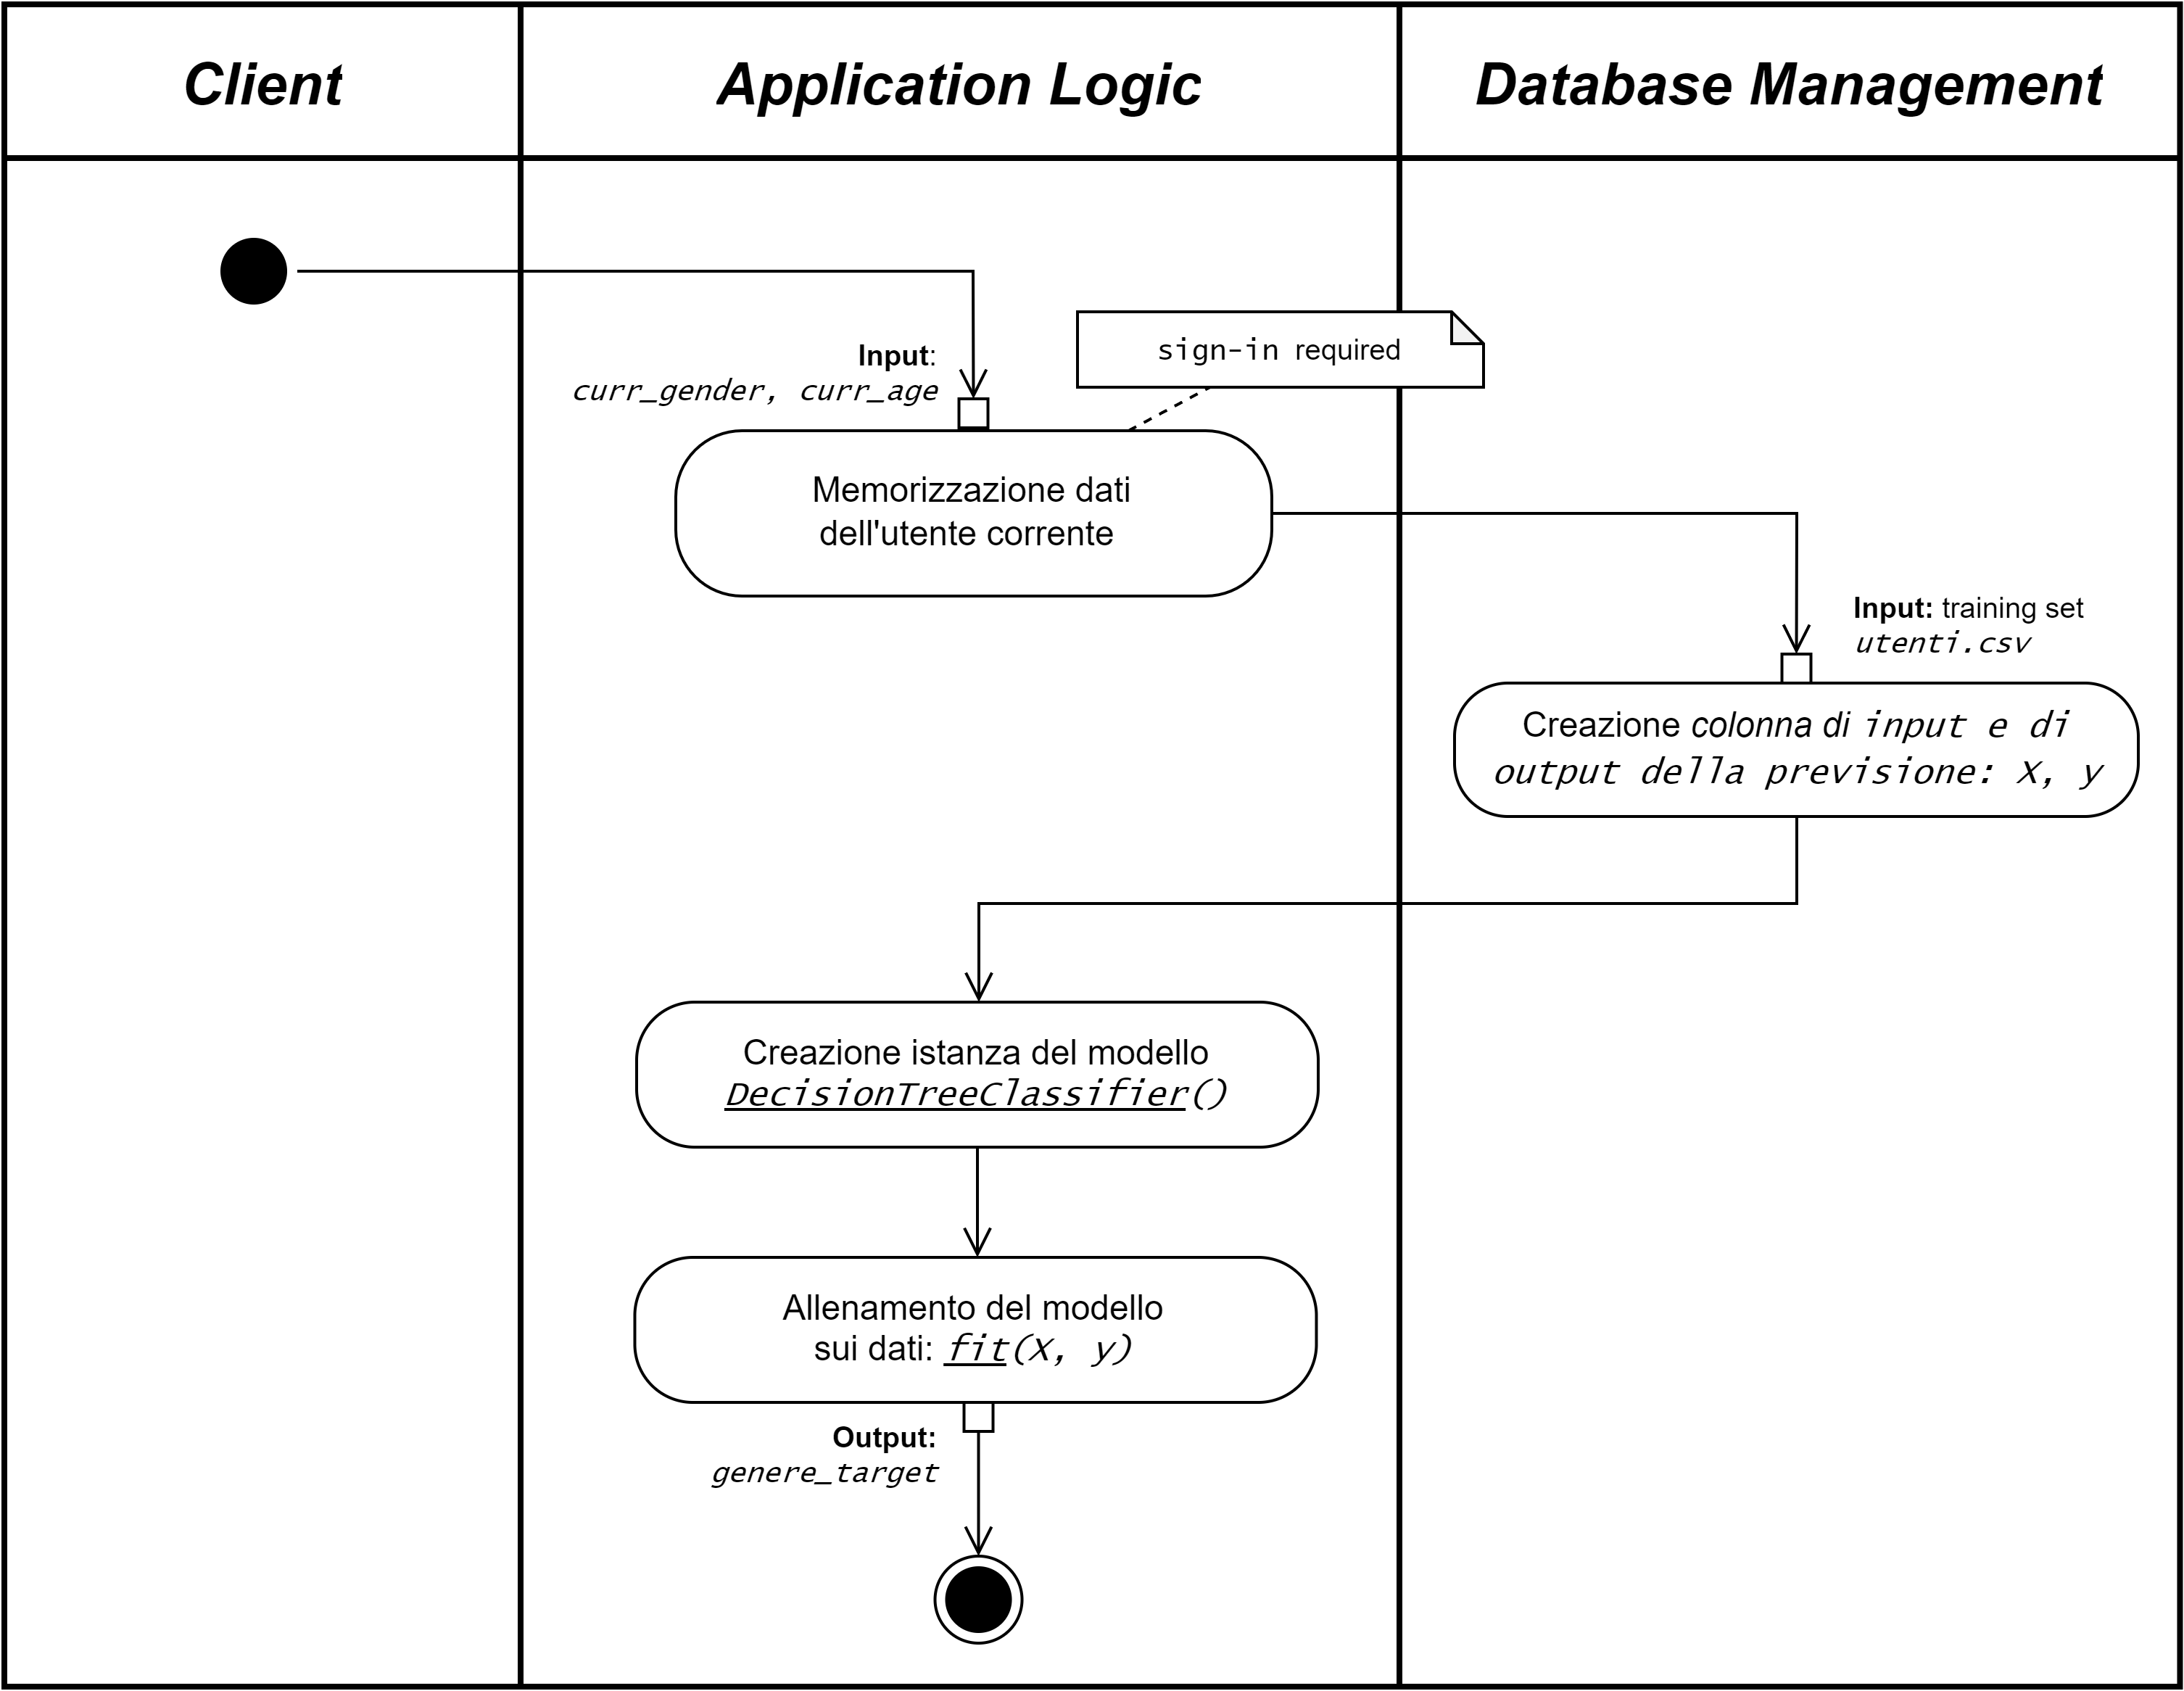
\includegraphics[scale=0.7]{images/flowchart_1_UML_ver2.png}
    \caption{UML Activity Diagram (parte I)}
    \label{fig-uml-ac-1}
\end{figure}


\newpage
\subsection{Algortimo Parte II}
\subparagraph{Pseudocodice}
%codice parte 2
Pseudocodice della seconda parte dell'algoritmo, relativa al suggerimento 
dei brani in base al genere target.
%\begin{figure}[H]
%    \centering
%    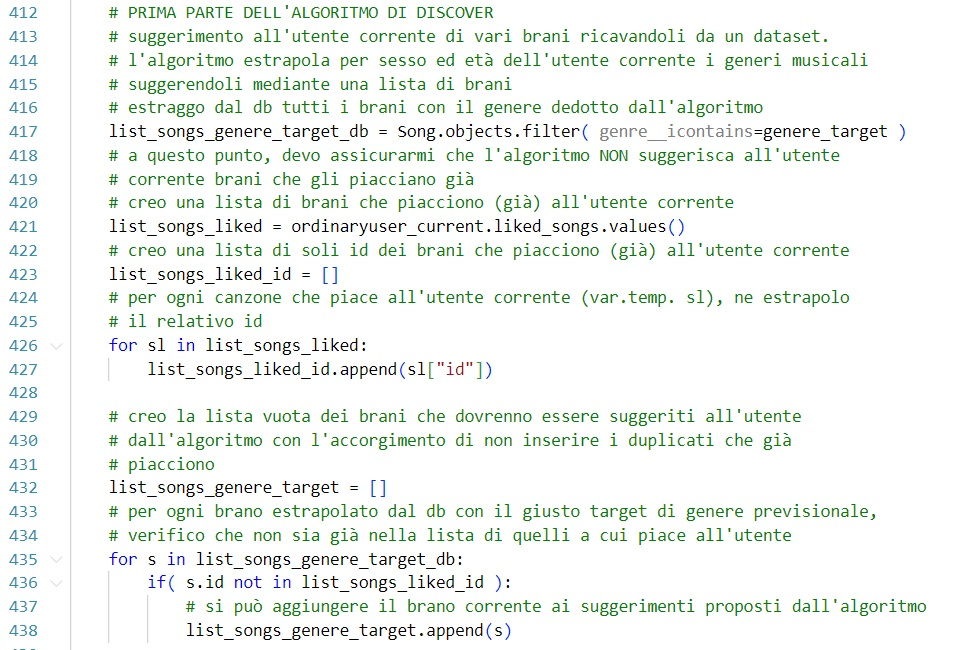
\includegraphics[scale=0.5]{images/alg2_v2.jpg}
%    \caption{Codice (parte II)}
%    \label{fig-codice2}
%\end{figure}
% pseudocodice 2
\begin{algorithm}
    \caption{Step 2 - Brani}
    \SetAlgoLined
    \SetKwProg{myalg}{algoritmo}{ begin}{end}
    \myalg{Discover($curr\_gender$, $curr\_age$)}{
        \BlankLine
        \textbf{...}
        \BlankLine
        \textbf{/* Estrazione dei brani con genere target */}\

        \textbf{do}{
            $songs\_list\_db \leftarrow Songs.\underline{filter}(genere=genere\_target)$
        }
        \BlankLine
        \BlankLine
        \textbf{/* Creazione lista dei brani che piacciono all'utente */}\

        \textbf{do}{
            $liked\_songs\_list \leftarrow curr\_user.liked\_song.\underline{values}()$
        }
        \BlankLine
        \BlankLine
        \textbf{/* Creazione lista vuota per gli id */}\

        \textbf{do}{
            $liked\_songs\_list\_id \leftarrow [] $
        }
        \BlankLine
        \BlankLine
        \textbf{/* Inserimento degli ID nella lista */}\

        \For{sl in liked\_songs\_list}{
            $liked\_songs\_list\_id.\underline{append}(sl[id])$
            
        }
        \BlankLine
        \BlankLine
        \textbf{/* Creazione lista per i brani da suggerire all'utente*/}\

        \textbf{do}{
            $songs\_list \leftarrow [] $
        }
        \BlankLine
        \BlankLine
        \textbf{/* Creazione lista vuota per i brani da suggerire all'utente*/}\

        \For{s in songs\_list\_db}{
            \If{s.id not in liked\_songs\_list\_id}{
                $songs\_list.\underline{append}(s)$
            }
        }
        \BlankLine
        \Return{$songs\_list$}\\
        \textbf{...}
        \BlankLine
        \KwResult{Lista brani con genere target}
        \BlankLine
        %\vspace{0.5cm}   
    }
\end{algorithm}
%flowchart 2
\newpage
%\subparagraph{Diagramma di flusso}
%Diagramma di flusso della seconda parte dell'algoritmo.
%\begin{figure} [H]
%    \centering
%    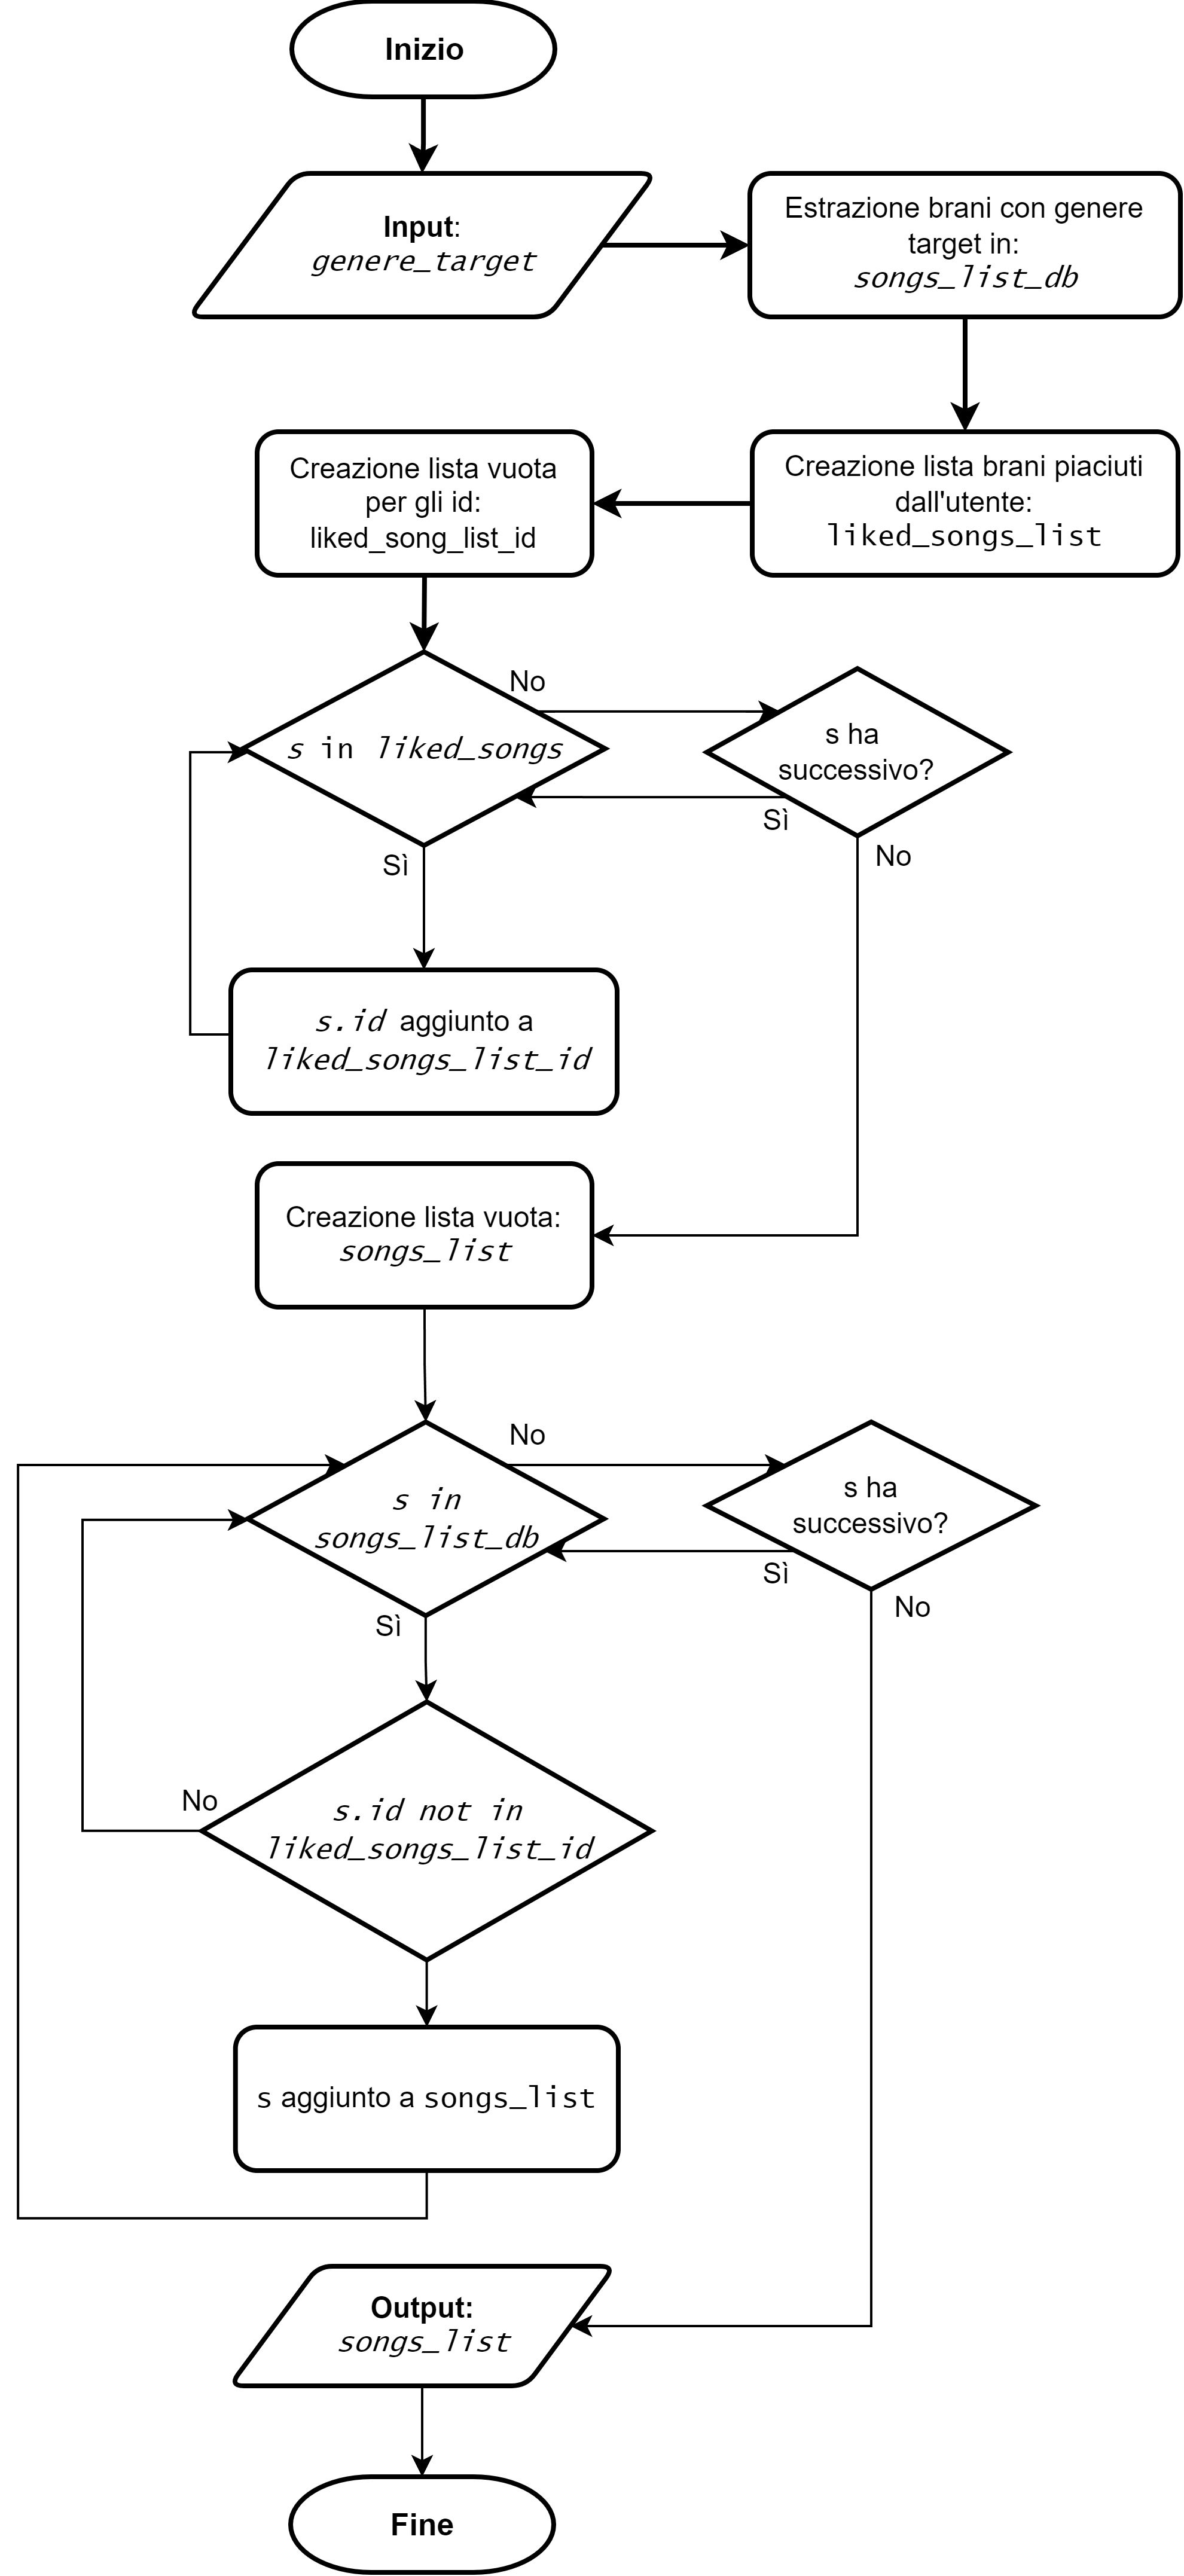
\includegraphics[scale=0.62]{images/flowchart-Parte II.png}
%    \caption{Flowchart (parte II)}
%    \label{fig-fc2}
%\end{figure}
\subparagraph{UML Activity Diagram}
Diagramma delle attività della seconda parte dell'algoritmo.
\begin{figure} [H]
    \centering
    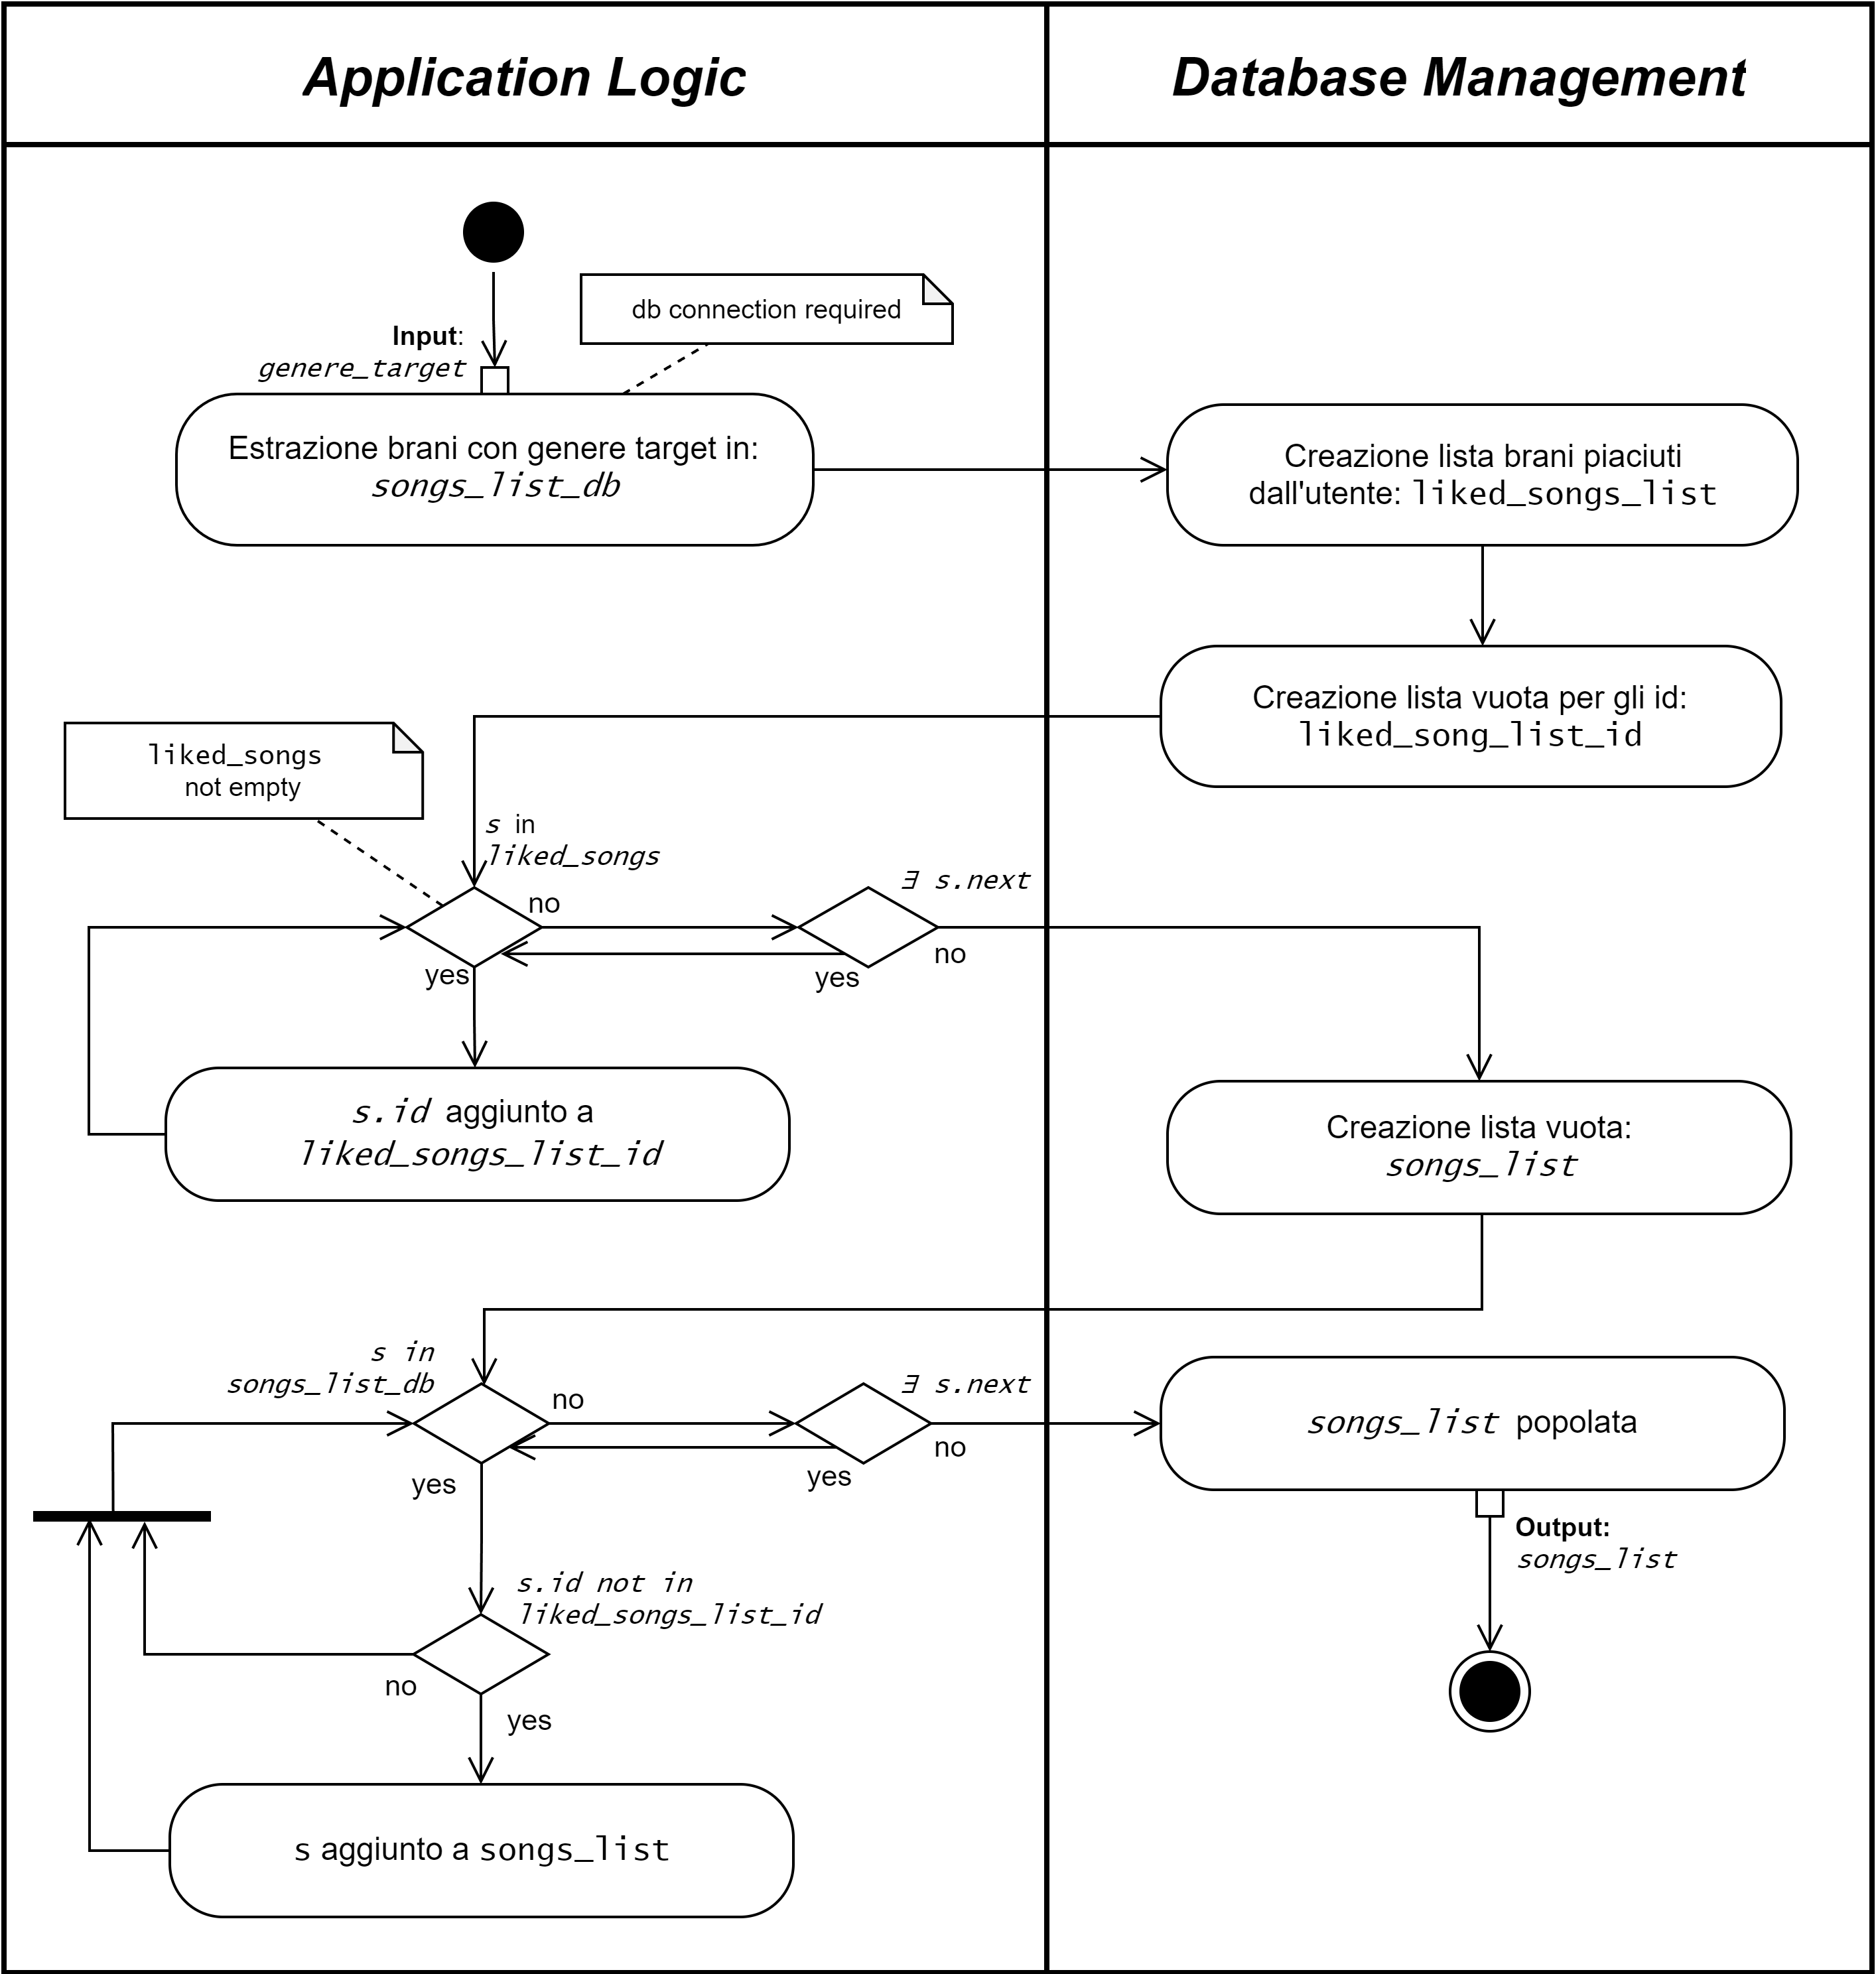
\includegraphics[scale=0.75]{images/flowchart_2_UML_ver2.png}
    \caption{UML Activity Diagram (parte II)}
    \label{fig-uml-ac-2}
\end{figure}




\newpage
\subsection{Algoritmo Parte III}

% codice 3
\subparagraph{Pseudocodice}
Pseudocodice della terza parte dell'algoritmo, quella relativa al
suggerimento di utenti con gusti simili. 
%\begin{figure}[H]
%    \centering
%    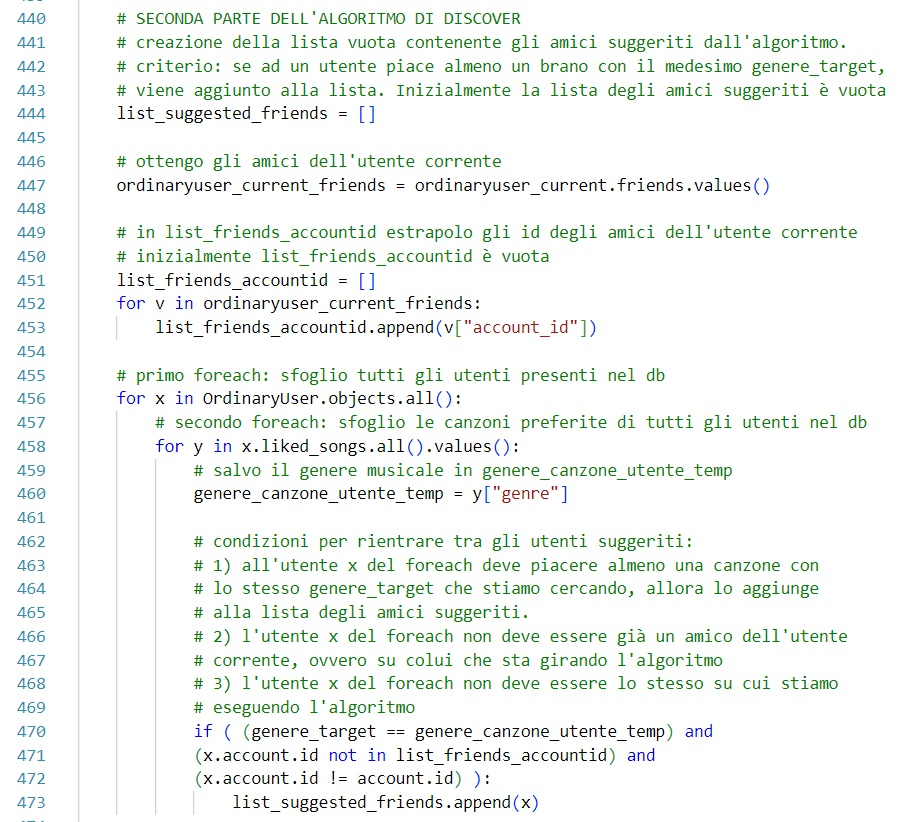
\includegraphics[scale=0.7]{images/alg3_v2.jpg}
%%    \caption{Codice (Parte III)}
%    \label{fig-codice3}
%\end{figure}


% pseudocodice 3
\begin{algorithm}
    \caption{Step 3 - Amici}
    \SetAlgoLined
       \SetKwProg{myalg}{algoritmo}{ begin}{end}
    \myalg{Discover($curr\_gender$, $curr\_age$)}{
        \BlankLine
        \textbf{...}
        \BlankLine
        \textbf{/* Creazione lista vuota */}\\
        \textbf{do}{
            $[] \leftarrow list\_suggested\_friends $
        }

        \BlankLine
        \BlankLine
        \textbf{/* Memorizzazione della lista di amici dell'utente*/}\\
        \textbf{do}{
            $friends\_id \leftarrow curr\_user.friends.\underline{values}() $
        }

        \BlankLine
        \BlankLine
        \textbf{/* Creazione lista vuota */}\\
        \textbf{do}{
            $[ ] \leftarrow list\_user\_friends $
        }


        \BlankLine
        \BlankLine
        \For{v in friends\_id }{
            %\tcp{Blocco di istruzioni da eseguire per ogni valore di i}
            $list\_user\_friends.\underline{append}(v[id])$
            
        }
        \BlankLine
        \textbf{/* Memorizzazione amici dell'utente corrente */}\\
        \ForEach{ x in user.\underline{all}()}{
            \ForEach{y in x.liked\_songs.\underline{all}().\underline{values}()}{
                $genere\_temp \leftarrow y [genere] $\\
                \If{genere\_target = genere\_temp AND x.account.id != account.id AND x.account.id not in list\_user\_friends }{
                    list\_suggested\_friends.\underline{append}(x)
                }
            }
        }
    \BlankLine
    \Return{list\_suggested\_friends}\\
    \textbf{...}
    \BlankLine
    \KwResult{Lista utenti con gusti affini all'utente}
    \BlankLine
    }
\end{algorithm}

% flowchart 3
\newpage
%\subparagraph{Diagramma di flusso} 
%Diagramma di flusso della terza parte dell'algoritmo.
%\begin{figure} [H]
%    \centering
%    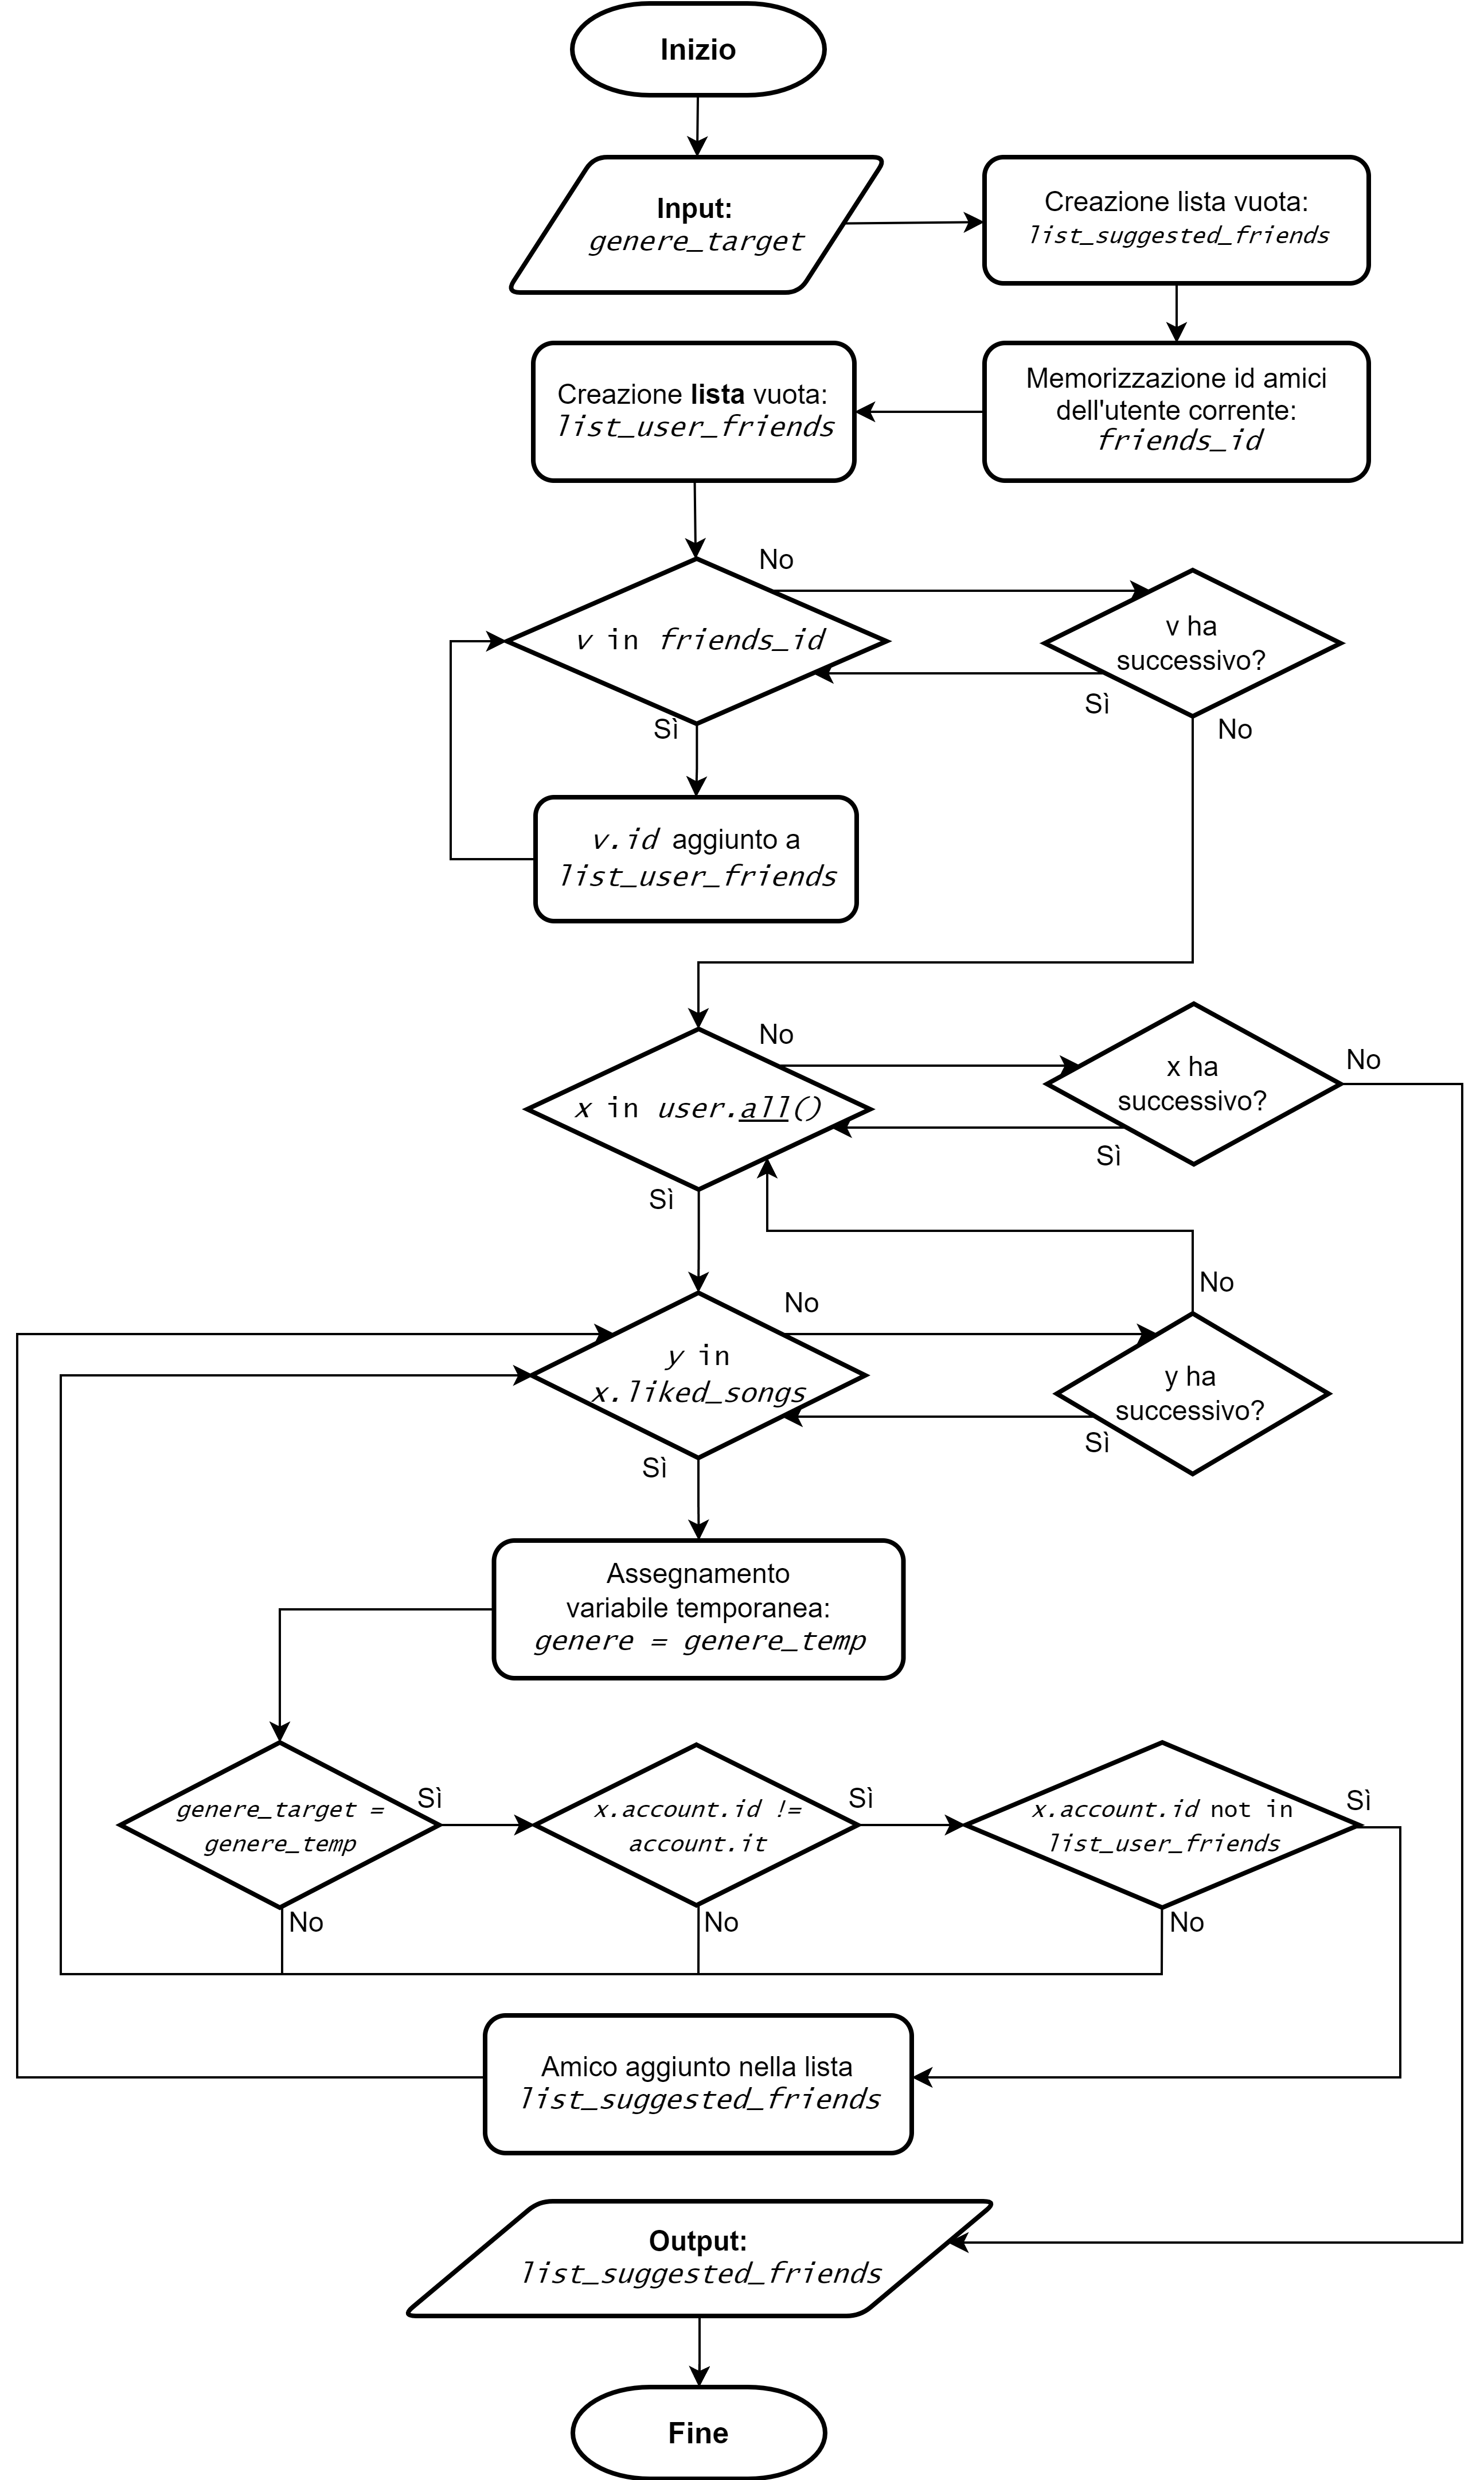
\includegraphics[scale=0.65]{images/flowchart-Parte III.png}
%    \caption{Flowchart (parte III)}
%    \label{fig-fc3}
%\end{figure}

\subparagraph{UML Activity Diagram}
Diagramma delle attività della terza parte dell'algoritmo.
\begin{figure} [H]
    \centering
    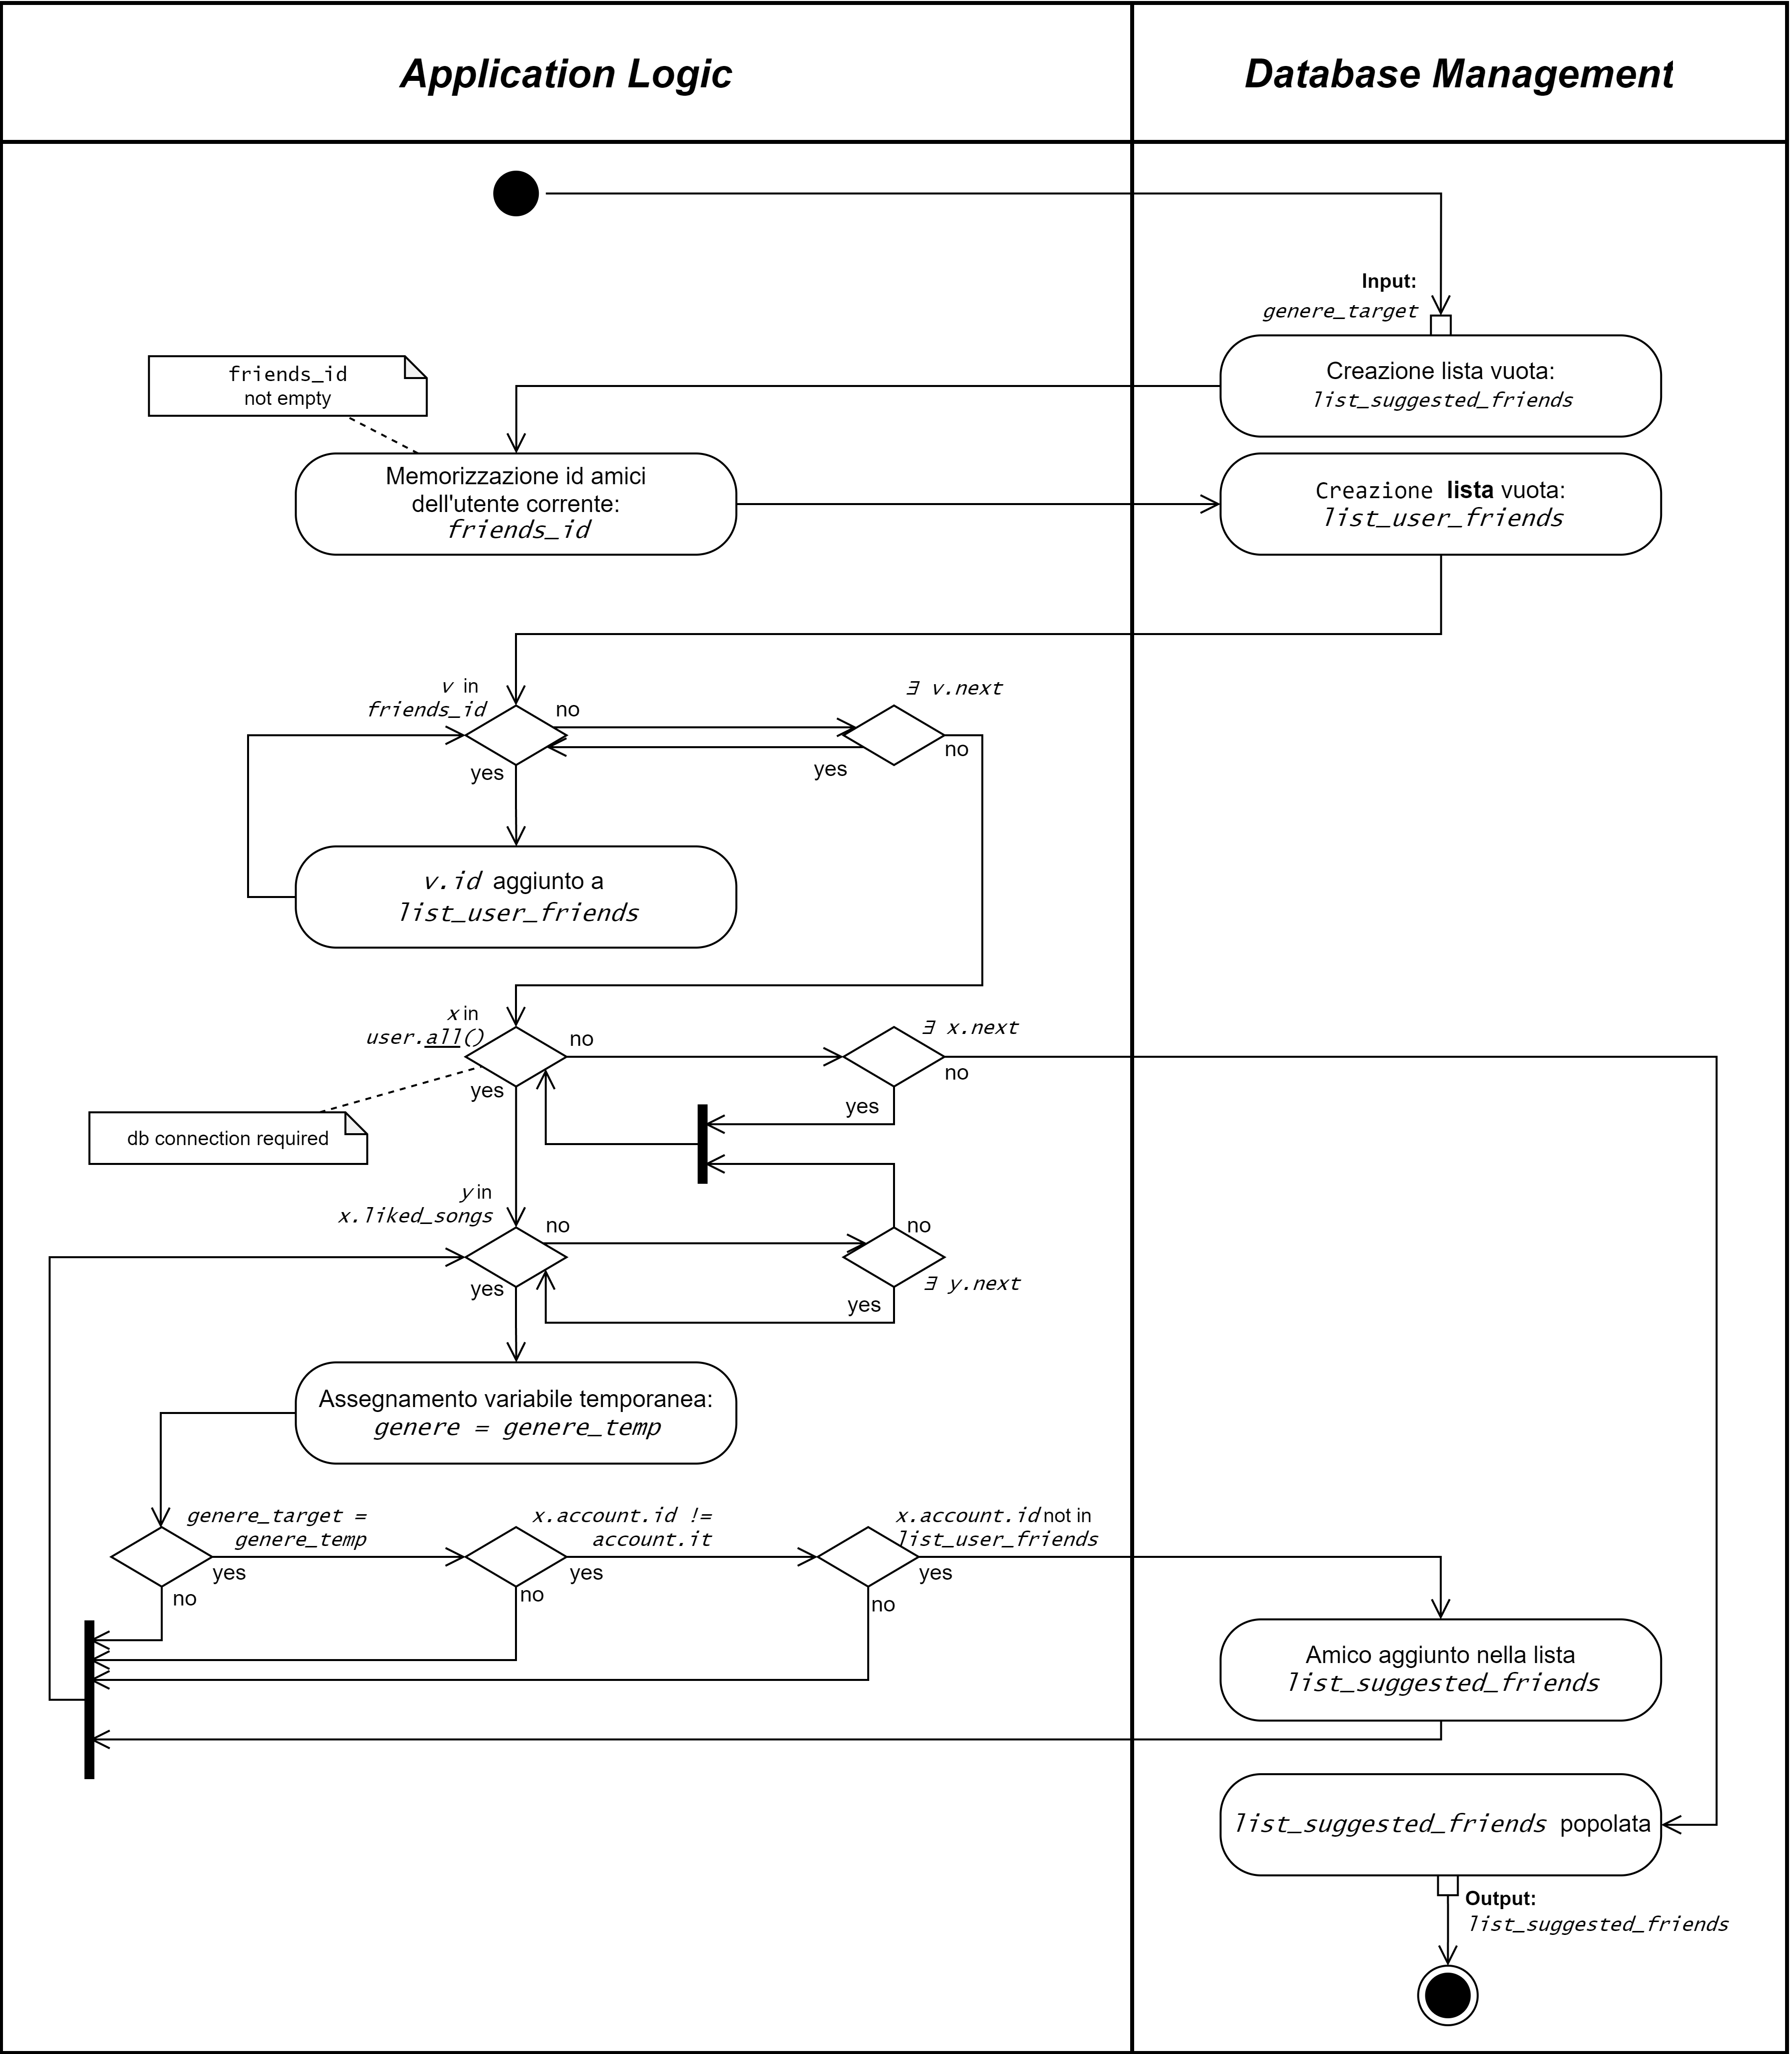
\includegraphics[scale=0.59]{images/flowchart_3_UML_ver2.png}
    \caption{UML Activity Diagram (parte III)}
    \label{fig-uml-ac-3}
\end{figure}



\newpage
\subsection{Algoritmo Parte IV}
% codice 4

\subparagraph{Pseudocodice}
Pseudocodice dell'ultima parte dell'algoritmo.  
%\begin{figure}[H]
%    \centering
%    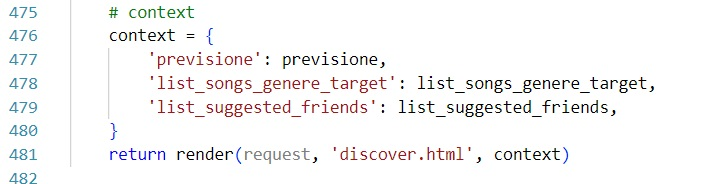
\includegraphics[scale=0.7]{images/alg4_v2.jpg}
%    \caption{Codice (parte IV)}
%    \label{fig-codice4}
%\end{figure}
%\vspace{0.5cm}

% pseudocodice 4
\begin{algorithm}

    \caption{Step 4 - Parametri di ritorno}
    \SetAlgoLined
   
    \SetKwProg{myalg}{algoritmo}{ begin}{end}
    \myalg{Discover($curr\_gender$, $curr\_age$)}{
        \BlankLine
        \BlankLine
        \textbf{...}
        \BlankLine
        \BlankLine
        \textbf{/* Ritorno parametri di interesse */}\\
        \Return{songs\_list}\\
        \Return{list\_suggested\_friends}\\    
        \BlankLine
        \BlankLine
        \KwResult{Lista brani con genere target e lista utenti con gusti affini all'utente }
        \vspace{0.5cm}
        %\label(alg:1)
    }
\end{algorithm}
% flowchart 4
\vspace{1cm}
%\subparagraph{Diagramma di flusso} Diagramma di flusso dell'ultima parte dell'algoritmo.
%\begin{figure} [H]
%    \centering
%    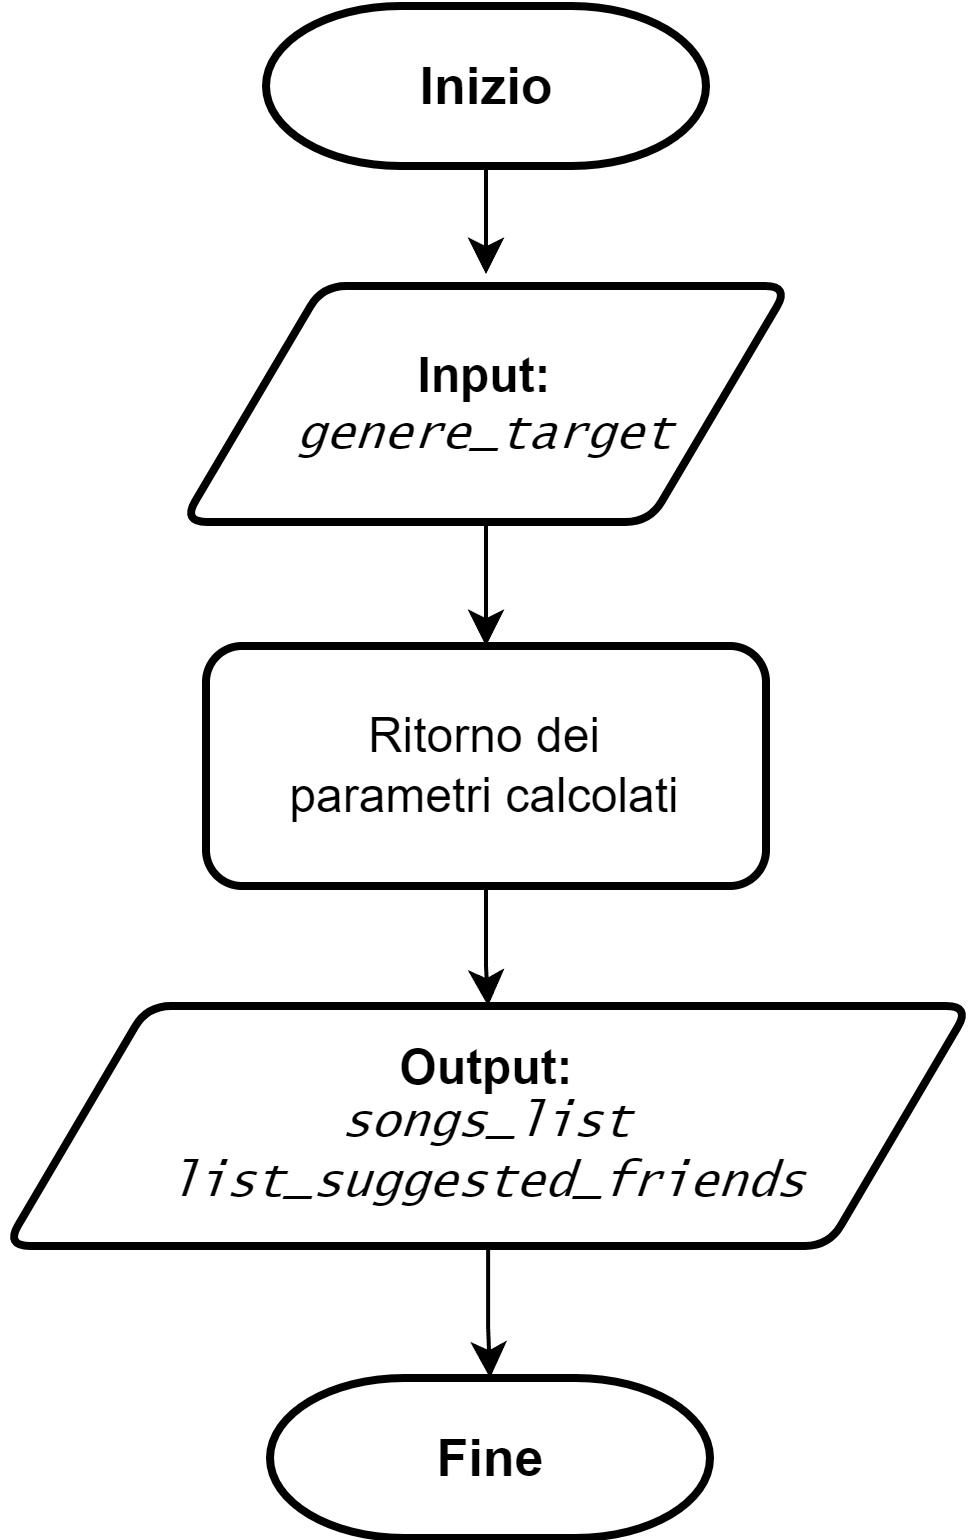
\includegraphics[scale=0.7]{images/flowchart-Parte IV.png}
%    \caption{Flowchart (parte IV)}
%    \label{fig-fc4}
%\end{figure}
\subparagraph{UML Activity Diagram}
Diagramma delle attività della parte finale dell'algoritmo.
\vspace{0.3cm}
\begin{figure} [H]
    \centering
    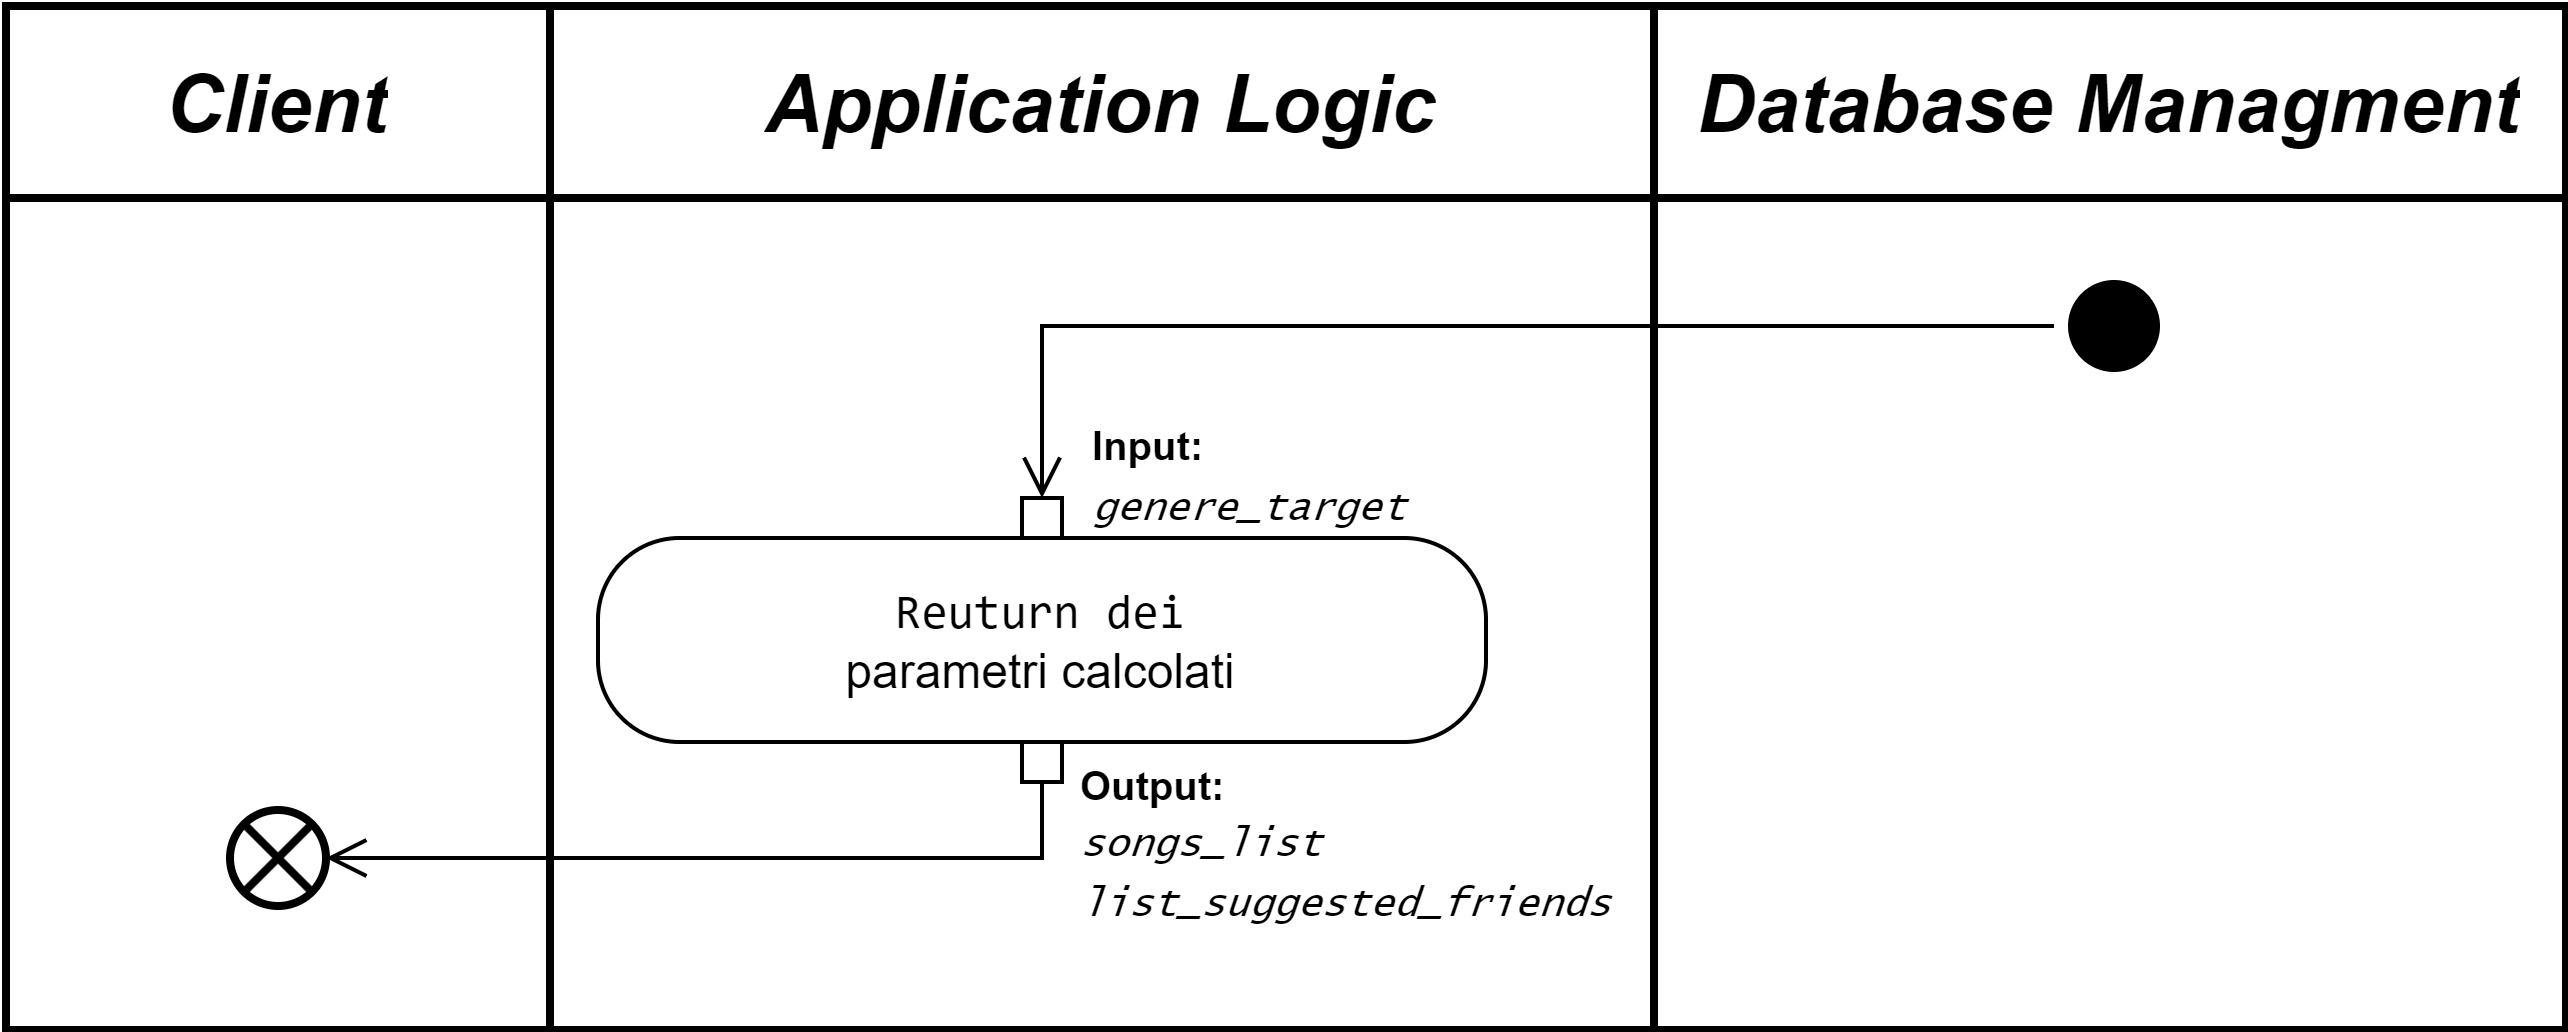
\includegraphics[scale=0.8]{images/flowchart_4_UML_ver2.png}
    \caption{UML Activity Diagram (parte IV)}
    \label{fig-uml-ac-4}
\end{figure}




\newpage
\subsection{Analisi della complessità}
Per valutare la complessità temporale dell'algoritmo, vengono esaminate le operazioni principali che 
vengono eseguite e e viene analizzato come queste operazioni dipendono dalla dimensione dell'input. 
Di seguito viene fornita una stima approssimativa della complessità temporale per ogni parte dell'algoritmo:

\begin{itemize}
    \item \textbf{Lettura del file CSV:} La lettura del file CSV tramite la funzione $read\_csv$ ha una 
    complessità temporale che dipende dalla dimensione del file, nello specifico dal numero di righe e colonne del file.
    Supponiamo che ci siano n righe e m colonne nel file. La lettura del file richiede un'operazione 
    per ogni cella nel file, di conseguenza la complessità è dell'ordine di ${O(n*m)}$.
    % sono 21 righe e 3 colonne, quindi può essere considerata costante O(1)
    \item \textbf{Creazione e addestramento del modello di classificazione:} La creazione del modello 
    \textit{DecisionTreeClassifier} e l'addestramento del modello tramite il metodo \textit{fit} dipendono dal numero di 
    caratteristiche e dal numero di esempi nel set di dati. Se denotiamo con p il numero di istanze (quindi n, le righe del file csv) 
    e con q il numero di attributi (m, il numero di colonne), allora la complessità temporale può essere approssimata a $O(p * q log(p))$, 
    poiché la costruzione di un albero decisionale richiede operazioni che dipendono da entrambi i valori.
    % sono 21 istanze e 3 colonne, quindi può essere approssimato a O(1) costante
    \item \textbf{Previsione dei generi musicali:} La previsione dei generi musicali per 
    l'utente corrente utilizzando il modello addestrato ha una complessità temporale di 
    $O(1)$, poiché si tratta di un singolo esempio (operazione costante).
    \item \textbf{Filtraggio dei brani musicali:} Per ogni brano che piace all'utente corrente, viene estratto il relativo
     ID e memorizzato in una lista. Questa operazione richiede un'iterazione su tutti i $s$ brani preferiti, quindi la 
     complessità è $O(s)$.
     Il filtro dei brani musicali nel database attraverso la chiamata 
    a \textit{Song.objects.filter} può dipendere dal numero di brani nel database e dalla complessità della query. 
    Questa operazione ha una complessità temporale dell'ordine di $O(s)$, dove s rappresenta il 
    numero di brani che soddisfano i criteri di filtro.
    \item \textbf{Creazione della lista dei brani suggeriti:} Per ogni brano del training set con il genere musicale dedotto
    dall'algoritmo, viene verificato se l'ID del brano non è presente nella lista dei brani preferiti dall'utente corrente. 
    Poiché questa operazione richiede l'iterazione su tutti i z brani nel training set, la complessità è $O(z)$.
    \item \textbf{Ricerca degli amici suggeriti:} La ricerca degli amici suggeriti coinvolge \textit{due cicli for nidificati}. 
    Supponendo che ci siano \textit{x} utenti nel database e \textit{y} canzoni preferite per ogni utente, la complessità temporale di questa
    parte dell'algoritmo può essere approssimata a $O(x * y)$.
    \item \textbf{Creazione del contesto:} La creazione del contesto finale ha una complessità temporale trascurabile, 
    poiché coinvolge solo l'assegnazione di variabili.
\end{itemize}
Quindi, sommando tutte queste parti, si può concludere che la complessità temporale complessiva dell'algoritmo 
è approssimativamente:

\boldmath
\begin{center}
    $O(n * m) + O(n * m log(m)) + O(s) + O(z) + O(x * y) + O(1)$
\end{center}
\unboldmath


\subparagraph{Analisi complessità di \textit{DecisionTreeClassifier}}
Il DecisionTreeClassifier fa parte di una libreria Python per il Machine Learning.
L'addestramento di un albero decisionale utilizzando DecisionTreeClassifier si basa 
su una serie di divisioni dei dati in base alle caratteristiche (features) dei campioni.
La complessità principale dell'addestramento di un albero decisionale è determinata 
dalla fase di costruzione dell'albero stesso.
Alberi decisionali sono metodi di learning supervisionato non parametrici usati per la classificazione
e la regressione. L'obiettivo è di creare un modello che preveda il valore di una variabile target tramite 
apprendimento di semplici regole decisionali e dedotte dalle caratteristiche dei dati. Quindi 
un albero può essere visto come una costantr approssimazione a tratti.


La complessità dell'addestramento di un albero decisionale è influenzata 
principalmente da due fattori:
\begin{itemize}
    \item Il numero di campioni nel set di addestramento (n): Più campioni ci sono, 
        più operazioni di divisione e valutazione devono essere eseguite.
    \item Il numero di caratteristiche (features) dei campioni nel set di addestramento (m): 
        Più caratteristiche ci sono, più divisioni devono essere valutate.
\end{itemize}

\vspace{0.3cm}
\subparagraph{Analisi complessità di \textit{fit}}
Il metodo fit in Pandas viene utilizzato per adattare un modello ai dati; in questo caso,
consente di produrre un modello di regressione lineare, insieme alla funzione analizzata
precedentemente. 
\vspace{0.5cm}


In conclusione, la complessità dell'addestramento di un albero decisionale 
con la funzione DecisionTreeClassifier e la regressione tramite fit 
risulta $O(n * m * log(m))$.






\newpage
\section{Analisi statica}
\vspace{2pt}
\subsection{Backend}
Il testing statico dei campi è una pratica comune nel processo di sviluppo del software 
per verificare che i dati immessi in determinati campi rispettino determinate regole o vincoli. 
Per l'analisi statica del back-end è stato usato pylint, un linter configurabile per il 
linguaggio Python. Esso mette a disposizione varie funzionalità:
\begin{itemize}
    \item imposizione di \textit{coding standard} e di \textit{code style};
    \item \textit{error detection}, sia a livello sintattico sia a livello di tipi;
    \item \textit{refactoring} per codice non usato e/o duplicato;
    \item integrazione con vari IDE al fine di fornire tutto ciò in tempo reale. 
\end{itemize}
Pylint è configurato tramite un file che contiene tutti parametri e le impostazioni 
da noi scelti per diminuire la complessità del codice ed aumentarne la chiarezza.
Il linting del progetto avviene tramite uno script e, oltre a warning ed errori, 
nell'output è presente anche un singolo numero (su una scala da 1 a 10) che valuta il codice. 
In particolare, alla fine di questa iterazione questo valore è pari a \textbf{9.18/10}.


\newpage
\section{Analisi dinamica}
\subsection{Testing Backend}
Durante la terza iterazione sono stati sviluppati dei test su specifici campi delle classi, organizzati nel file test.py. Per supportare l'esecuzione 
dei test, sono state create funzioni ausiliarie raggruppate nel file utility.py.
Di seguito vengono descritti i casi di test per i campi chiave delle classi Account, Album e Playlist.

\vspace{3pt}
\subparagraph{Test per la classe \textbf{Account:}} La classe Account gestisce le informazioni dell'utente, come il nome e l'email. 
Durante la fase di registrazione, sono presenti diversi casi di test che verificano la validità dei dati immessi.
I test riportati di seguito verificano che il nome e l'email immessi durante la registrazione non siano vuoti. 
Se il nome è vuoto o contiene un numero, o se la email non è stata dichiarata correttamente, i test restituiscono false, altrimenti restituiscono true.

\vspace{3pt}
\begin{lstlisting}   
def test_name_account_empty(self):
    name_fake = ``''
    account_fake = Account(name = name_fake)
    self.assertIs(account_fake.account_name_correct(), 
                                                False)
\end{lstlisting} 

\vspace{3pt}
%\begin{lstlisting}[caption={class AccountModelTests(TestCase)}, captionpos=b]

\begin{lstlisting}
def test_name_account_number(self):
    name_err = ``Luca''
    account_err = Account(name = name_err)
    self.assertIs(account_err.account_name_correct(), 
                                                False)
\end{lstlisting} 

\vspace{3pt}
\begin{lstlisting}
def test_email_account_correct(self):
    email_fake = ``pulcinopiowemusic.it''
    account_fake = Account(email = email_fake)
    self.assertIs(account_fake.account_email_correct(), 
                                                False)
\end{lstlisting}


\newpage
\vspace{5pt}
\subparagraph{Test per la classe \textbf{Song:}} La classe Song include le informazioni relative al brano. Di seguito sono riportati alcuni dei casi di test effettuati.
I test riportati di seguito verificano che il nome e il genere immessi durante la creazione del brano siano validi. 
Se i campi non rispettano determinati criteri o restrizioni, i test restituiscono false, altrimenti restituiscono true.
\vspace{3pt}
%\begin{lstlisting}[caption={class SongModelTests(TestCase)}, captionpos=b]

\begin{lstlisting}
    def test_song_title_correct(self):
    title_ok =``La primavera''
    song_fake = Song(title=title_ok)
    self.assertIs(song_fake.song_title_correct(), True)
\end{lstlisting} 
\vspace{3pt}
\begin{lstlisting}
def test_song_genre_correct(self):
    genre_err = ``arabasound''
    genre_err = Song(genre=genre_err)
    self.assertIs(genre_err.song_genre_correct(), 
                                            False)
\end{lstlisting}

\vspace{5pt}
\subparagraph{Test per la classe \textbf{Playlist:}} La classe Playlist include le informazioni di una playlist musicale. È presente un caso di test che verifica la validità del nome della playlist:
I test riportati di seguito verificano che il nome e la data immessi durante la creazione della playlist siano validi. 
Se il nome non rispetta determinati criteri o restrizioni, o se la data non rispetta un formato o una logica valida, i test restituiscono false, altrimenti restituiscono true.

\vspace{3pt}
%\begin{lstlisting}[caption={PlaylistModelTests(TestCase)}, captionpos=b]

\begin{lstlisting}
def test_playlist_name_correct(self):
    playlist_name_empty = ``"
    playlist_err = Playlist(name = playlist_name_empty)
    self.assertIs(playlist_err.playlist_name_correct(), 
                                                False)
\end{lstlisting} 

\vspace{3pt}
\begin{lstlisting}
def {test_playlist_creation_date_correct(self)}:
    playlist_creat_date_err = timezone.now() + 
                        datetime.timedelta(days=30)
    playlist_err = Playlist(creation_date=
                            playlist_creat_date_err)
    self.assertIs(playlist_err.playlist_creation_date_
                                    correct(), False)
\end{lstlisting} 



\newpage
\subparagraph{Test per la classe \textbf{Album:}} La classe Album include le informazioni riguardanti un album musicale. 
Il test riportato di seguito verifica che la data di pubblicazione immessa per l'album sia valida. 
Se la data non rispetta un formato o una logica valida, il test restituisce false, altrimenti restituisce true.
\vspace{3pt}
%\begin{lstlisting}[caption={class AlbumModelTests(TestCase)}, captionpos=b]

\begin{lstlisting}
def test_album_data_pub_correct(self):
    time = timezone.now() +  datetime.timedelta
                                            (days=30)
    future_album = Album(pub_date = time)
    self.assertIs(future_album.album_pub_correct(), 
                                                False)
\end{lstlisting} 

\newpage
\subsection{Coverage}
Coverage.py è uno strumento atto a misurare la copertura del codice per il linguaggio
Python. È anche disponibile un output interattivo in HTML, il cui output per il codice di questa iterazione è visibile
in figura \ref{fig-coverage}.
\begin{figure} [H]
    \centering
    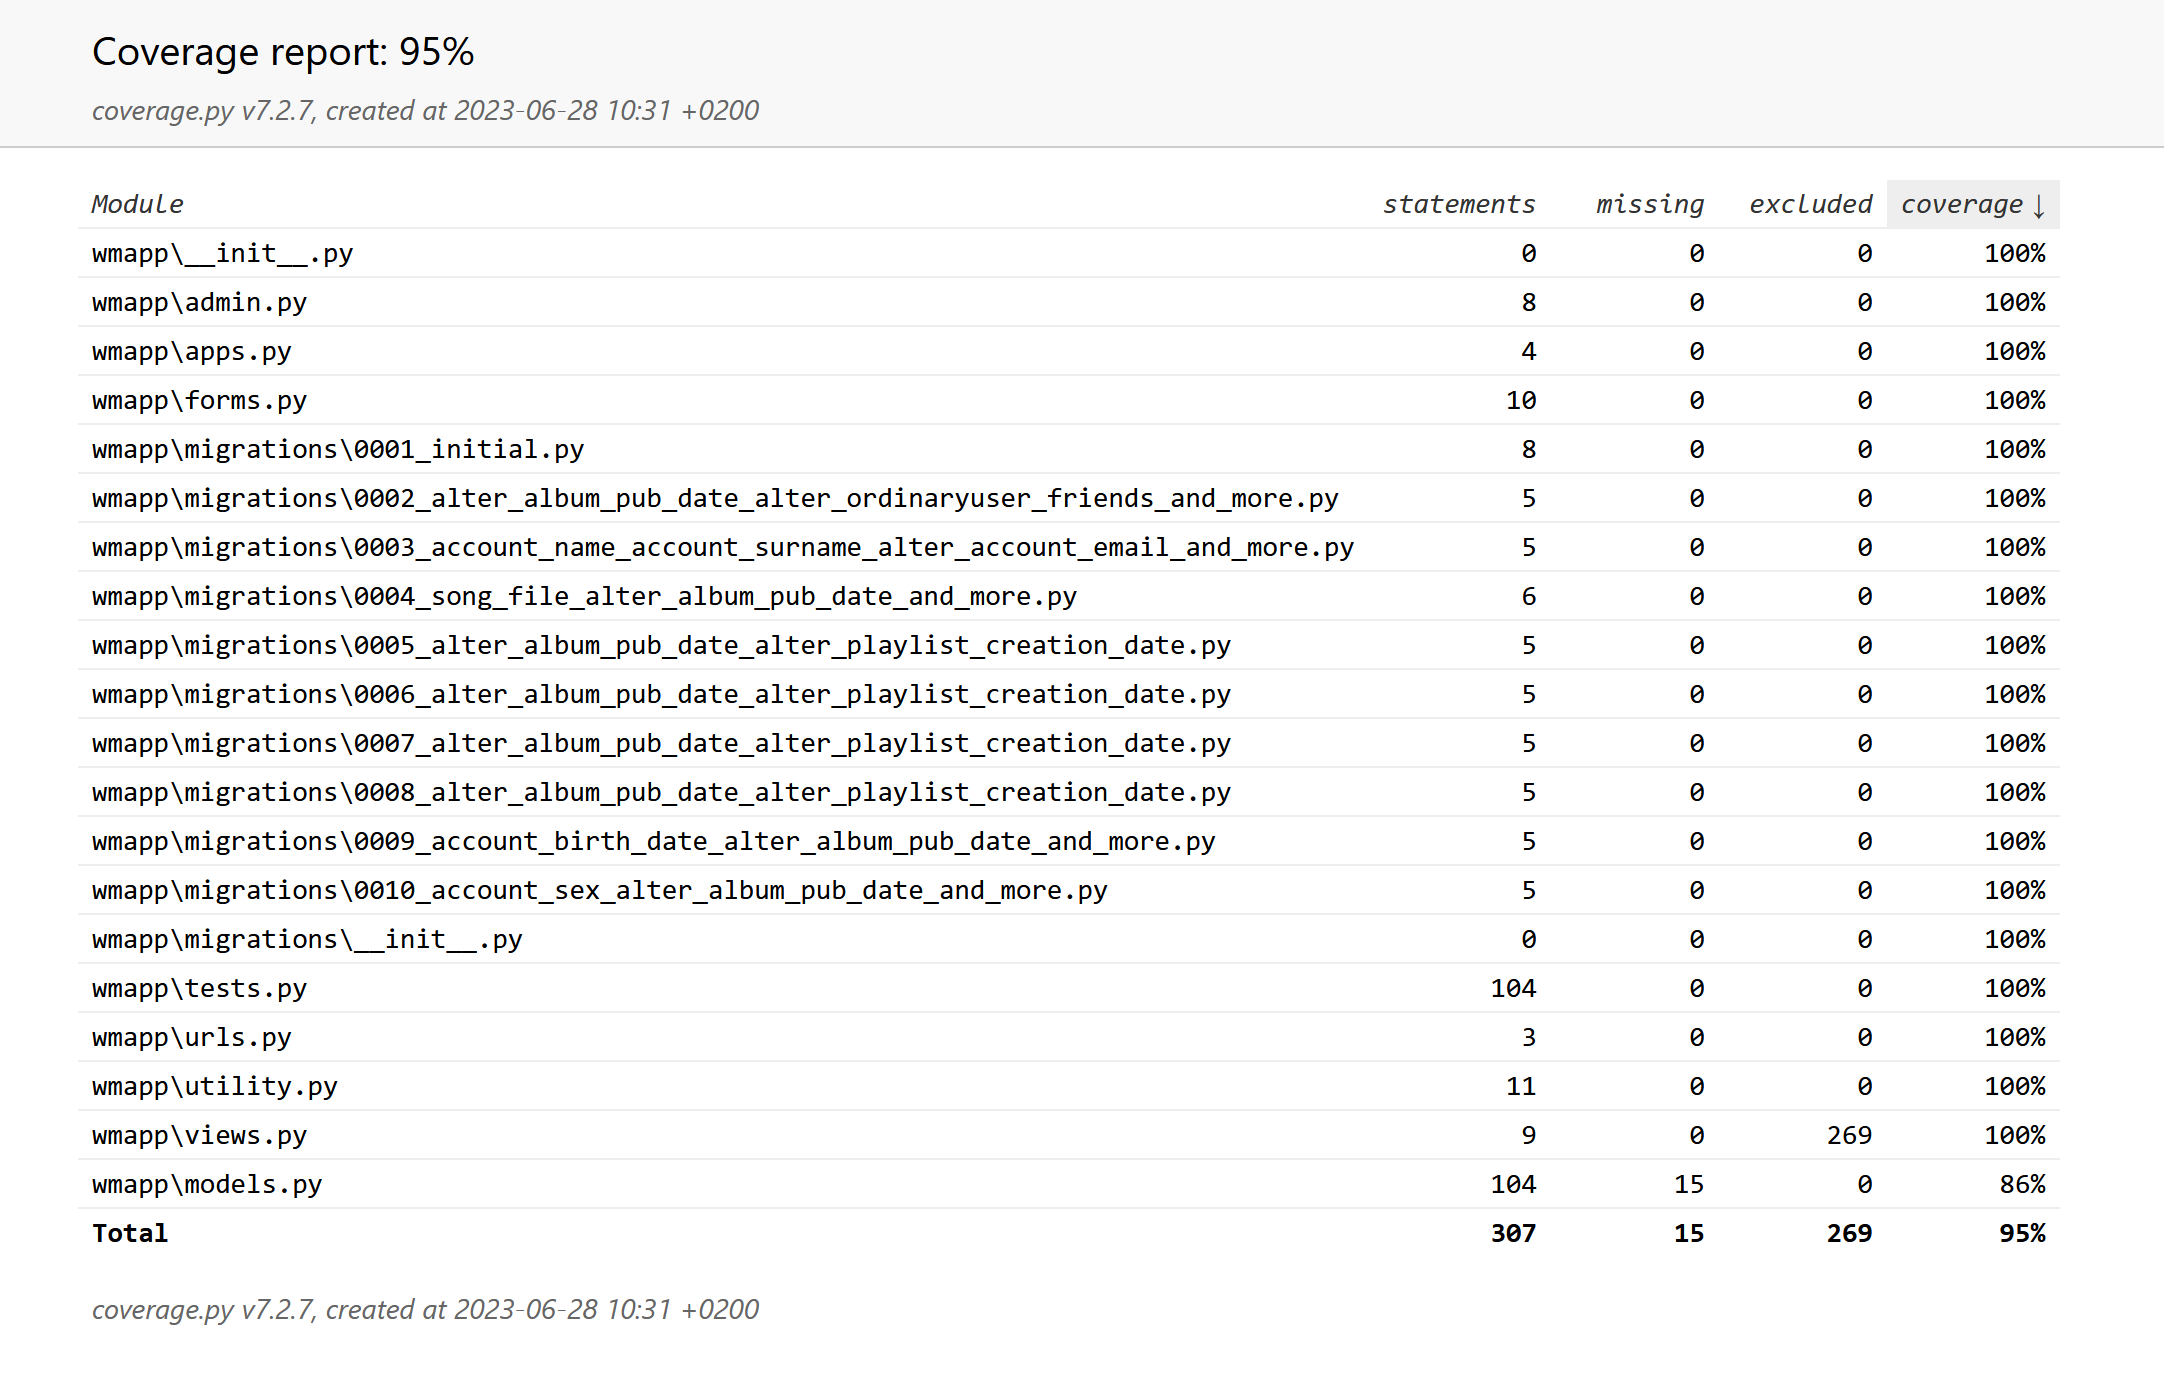
\includegraphics[scale=0.22]{images/coverage.png}
    \caption{Coverage.py results}
    \label{fig-coverage}
\end{figure}
